\chapter{Statistisk inferens:  Sannsynligheter og andeler}
\label{kap:sannsynligheter_og_andeler} % Opprinnelig kapittelnr: 7

\section{Innledning}
En stokastisk modell som inneholder nok antakelser til at vi kan
beregne sannsynligheten for enhver begivenhet i modellen, kalles
en {\em helspesifisert modell.} De modeller vi har studert
ovenfor i kapitlene om sannsynlighets\-regning har alle vært
helspesifiserte. I enkelte situasjoner kan vi være villige til å
gjøre en del antakelser, men ikke nok til at modellen blir
helspesifisert. Vi taler da om en {\em delvis spesifisert
modell}. I praksis støter vi ofte på problemstillinger hvor vi,
med utgangspunkt i en delvis spesifisert modell, ønsker å utføre
det eksperimentet som modellen er ment å beskrive, for om mulig å
finne ut noe om de uspesifiserte elementene i modellen. \\

\begin{eksempel}{Produksjonsprosess}
En produksjonsprosess skal produsere $n=100$ artikler. Vi er
villige til å gjøre følgende antakelser om prosessen:
\begin{enumerate}
 \item  Hver produsert artikkel blir enten defekt eller intakt.
 \item  Sannsynligheten $p$ for defekt er den samme for alle
          artikler.
\item   Uavhengighet.
\end{enumerate}
Dvs. at vi har en binomisk forsøksrekke. Dersom vi, f. eks. ut
fra tidligere erfaring, er villige til å anta at $p=0.10$, har vi
en helspesifisert modell. Det er da et rent
sannsynlighetsteoretisk problem å beregne sannsynligheten for en
hvilken som helst begivenhet som måtte interessere oss. Lar vi
for eksempel $X$ betegne antall defekte artikler, vet vi at

\[      X \mbox{\ \  er binomisk fordelt $(n=100, p=0.10)$.} \]

\noindent Uten noen slik antakelse om $p$, har vi bare en delvis
spesifisert modell. Vi har da ikke nok antakelser til å kunne
beregne sannsynligheter. Nå er

\[            X \mbox{\ \  binomisk fordelt $(n=100, p)$} \]

\noindent hvor $p$ er uspesifisert, dvs. (mer eller mindre) ukjent. Vi kan
da ønske oss nærmere opplysninger om $p$. For dette formål kan vi
gjennomføre produksjonen av de $n=100$ artiklene. På basis av den
delvis spesifiserte modellen og det observerte
produksjonsresultat, kan vi kanskje gi et brukbart anslag for $p$
({\em estimering}). Kan hende er problemstillingen den at man
ønsker å gå over til en ny produksjonsmetode. For den
tradisjonelle produksjonsmetoden er erfaringsvis $p=0.10$, mens
for den nye metoden er $p$ ukjent. På grunnlag av en
prøveproduksjon på $n=100$ artikler ønsker man å fastslå om
det er noen grunn til å påstå at den nye metoden gir bedre kvalitet
enn den gamle, dvs. påstå at $p<0.10$ ({\em hypotesetesting}).
Slike problemer er ikke lenger rene sannsynlighetsteoretiske
problemer, de er såkalte {\em statistiske inferensproblemer}.
\end{eksempel}

\begin{eksempel}{Utvalgsundersøkelse}
En forening har $N=$1000 medlemmer hvorav $M$ menn og $N-M$
kvinner. Det trekkes et tilfeldig utvalg på $n$=100 medlemskort.
Lar vi $Y$ betegne antall menn i utvalget, vet vi at

\[ Y  \mbox{\ \  er hypergeometrisk fordelt $(N=1000, M, n=100)$.} \]

\noindent Dersom antall mannlige medlemmer er kjent, f.eks. $M$=500, er
modellen helspesifisert, og sannsynligheten for begivenheter
vedrørende utvalget kan beregnes. For eksempel kan vi beregne
sjansen for at det er flere menn enn kvinner i utvalget. I fall
$M$ er ukjent, har vi bare en delvis spesifisert mo\-dell. Formålet
med å trekke et tilfeldig utvalg av medlemskort er kanskje
nettopp å finne ut noe om $M$, f.eks. klarlegge om det er flere
menn enn kvinner i foreningen. Vi har da ikke lenger et rent
sannsynlighetsteoretisk problem, men et statistisk
inferensproblem. \\
\end{eksempel}

Vi kan si at sannsynlighetsregning og statistisk inferens er
komplementære disipliner:\\

\noindent {\bf Sannsynlighetsregning:} Med utgangspunkt i en
     helspesifisert modell for et eksperiment kan vi, før
     eksperimentet utføres, beregne sannsynligheter for
     begivenheter vedrørende eksperimentet.\\

\noindent {\bf Statistisk inferens:} På bakgrunn av en delvis
     spesifisert modell for et eksperiment kan vi, på basis av
     det observerte utfall av eksperimentet, si noe om de
     uspesifiserte elementer i modellen. \\

Selv om vi i dette kapitlet i hovedsak er interessert i
statistisk inferens om sannsynligheter (Eksempel 1) eller andeler
(Eksempel 2), vil vi innføre en del generell teori som også
danner en vesentlig del av grunnlaget for neste kapittel.

\section{Estimering}
Anta at vi har en delvis spesifisert modell for et eksperiment,
der det uspesifiserte element vi er interessert i kan uttrykkes
ved en parameter $\theta$ hvis verdi er ukjent. I Eksempel 1 kan
f.eks. sannsynligheten $p$ være den ukjente parameter, dvs.
$\theta =p$. I Eksempel 2 kan det f.eks. være andelen $a$ av
menn i populasjonen, dvs. $\theta =a=M/N$. Vi ønsker på grunnlag
av det observerte utfall av eksperimentet å komme med et anslag,
i fagterminologien ofte kalt et {\em estimat}, for den ukjente
parameteren $\theta$. I Eksempel 1 virker det rimelig å bruke den
relative hyppighet av defekte i prøveproduksjonen som estimat for
den ukjente defektsannsynligheten. I Eksempel 2 vil andelen menn
i utvalget være et rimelig estimat for andelen menn i
populasjonen. Et slikt estimat kan treffe mer eller mindre godt, og vi
kan ikke på forhånd være sikker på hvor godt, estimater vil
vanligvis være underlagt tilfeldigheter. For å illustrere dette
poenget ser vi på et lett gjennomskuelig eksempel. \\

\begin{eksempel}{Myntkast}
Finn et kronestykke og forsøk å anslå sannsynligheten $p$ for at
et myntkast gir kron på grunnlag av $n=10$ myntkast (glem for en
stund at du vet at Norges Bank leverer mynter med $p=1/2$). Mitt
kronestykke ga bare 3 kron, og med denne opplysningen alene
velger jeg å estimere kronsannsynligheten med den relative
hyppigheten av kron, dvs. med $3/10=0.3$. I denne situasjonen er
det rimelig å anta at antall kron er binomisk fordelt $(n=10,p)$,
og i fall mynten er rettferdig var sjansen for at nettopp denne
estimerte verdi skulle slå til lik ca. $0.117$. De mulige verdier
med tilhørende sannsynligheter finner vi av Tabell~\ref{tab:Binomisk_fordeling_p05}:
\begin{center} \addtolength{\tabcolsep}{-0.3\tabcolsep}
\begin{tabular}{lcccccccc}
Estimert verdi: & 0.0 & 0.1 & 0.2 & 0.3 & 0.4 & 0.5 & 0.6 & $\ldots $ \\
Sannsynlighet:  &0.001& 0.010 & 0.044 & 0.117 & 0.205 & 0.246 & 0.205&$\ldots$
\end{tabular}
\end{center}
\noindent Når mynten er rettferdig $(p=0.5)$ vil 0.5 riktignok være den
estimerte verdi som har størst sjanse for å slå til, men risikoen
for store feilanslag er betydelig. Tilsvarende ser vi av Tabell~\ref{tab:Binomisk_fordeling}
at dersom vi hadde en falsk mynt med kronsannsynlighet
$p$=0.4, vil 0.4 være det mest sannsynlige estimat, med omtrent
samme risiko for feilanslag. For generelt å redusere risikoen for
feilanslag må vi selvfølgelig utføre et større antall myntkast.
Undersøker vi f.eks. tilfellet $n=100$ vil, dersom mynten er
rettferdig, fortsatt 0.5 være det estimat som har størst
sannsynlighet, mens sannsynligheten for å få et estimat som
avviker mye er redusert. Sannsynligheten for at estimert verdi
blir akkurat 0.5 er riktignok bare 0.08, men i tilfellet
$n=100$ er det langt flere mulige verdier omkring 0.5. Eksempelvis
blir sannsynligheten for at anslaget faller i intervallet fra
	0.45 til 0.55 lik 0.73 (se også Oppgave~\ref*{kap:sannsynlighetsfordelinger}.24). Samme
vurderinger kan gjøres dersom mynten er falsk.
\end{eksempel}

\begin{center} \framebox[10cm]{\begin{minipage}{9cm}\rule{0cm}{0.5cm}
\begin{definisjon}
     En {\em estimator} $\hat{\theta}$ for en
     ukjent parameter $\theta$ er en stokastisk variabel, der
     realisert verdi kan brukes som estimat (anslag) for $\theta$.
 \end{definisjon}
\end{minipage}} \end{center}

\noindent Et estimat for parameteren $\theta$ er brukbart når det er
 nær den faktiske verdi av $\theta$. Vi bør derfor velge en estimator
$\hat{\theta}$ som har stor sannsynlighet for å gi et estimat nær
$\theta$, uansett hvilken verdi $\theta$ måtte finne på å ha.
Dette innebærer at sannsynlighetsfordelingen (ofte kalt {\em
sampling-fordelingen}) til $   \hat{\theta}   $ bør være konsentrert
omkring den ukjente $\theta$. Vi har flere muligheter for å
uttrykke et slikt ønske, eksempelvis
\begin{enumerate}
\item  $E\mid \hat{\theta} - \theta \mid$         bør være liten
\item  $E(\hat{\theta} - \theta )^2$             bør være liten
\item  $P(\mid \hat{\theta} - \theta \mid <d)$    bør være stor.
\end{enumerate}
Her vil vi kalle $\mid \hat{\theta} - \theta \mid$ for estimeringsfeilen.
Nr. 1 ønsker seg liten forventet estimeringsfeil, mens nr. 2
ønsker seg liten forventet kvadrert estimeringsfeil. Nr. 3
ønsker, for gitt $d>0$, at sannsynligheten for estimeringsfeil
mindre enn $d$ skal være stor. I praksis viser det seg at det
første kriteriet er lite velegnet, og vi skal derfor studere de
to siste kriteriene. Følgende identitet er viktig (se Oppgave~14).

\[E({\hat{\theta}-\theta )}^2=var\hat{\theta}+{(E\hat{\theta}-\theta )}^2 \]

\noindent Vi ser at om forventet kvadratfeil $E{(\hat{\theta}-\theta )}^2$ skal
bli liten, må følgende to betingelser være oppfylt:
\begin{enumerate}
\item $E \hat{\theta} $ må avvike lite fra $\theta$.
\item $var \hat{\theta} $ må være liten.
\end{enumerate}
I mange situasjoner er det rimelig å velge en estimator $ \hat{\theta} $
som er slik at $E\hat{\theta} = \theta$, og vi innfører derfor følgende
begrep:

\begin{center} \framebox[10cm]{\begin{minipage}{9cm}\rule{0cm}{0.5cm}
 \begin{definisjon}
     En estimator $ \hat{\theta} $ sies å være {\em
     forventningsrett} for $\theta$ dersom $E\hat{\theta} =\theta$
     uansett $\theta$. En estimator som ikke er forventningsrett
     vil vi kalle {\em forventningsskjev}.
 \end{definisjon}
\end{minipage}} \end{center}
Vi ser at med en forventningsrett estimator $\hat{\theta}$, blir
 $E{(\hat{\theta}-\theta)}^2=var\hat{\theta} $, og en sammenligning av to
eller flere forventningsrette estimatorer kan derfor skje ved å sammenligne
deres varianser. Vi velger da den estimator som har minst varians.

La oss illustrere betraktningene ovenfor med eksempler: Anta at
vi har valget mellom to estimatorer kalt $\hat{\theta}$ og
 $\check{\theta}$ med
sannsynlighetsfordelinger (samplingsfordelinger) som på Figur~\ref{fig:samplingfordeling}.

\begin{figure}[ht]
\centering
\includegraphics[scale=0.8]{figurer/fig7_1.pdf}
    \caption{Samplingfordelinger til estimatorer $\hat{\theta}$ og $\check{\theta}$}
	\label{fig:samplingfordeling}
\end{figure}                                                               
\noindent I Figur~\ref{fig:samplingfordeling}a--b er $\hat{\theta}$ forventningsrett, mens
 $\check{\theta}$ er forventningsskjev. Siden $ \hat{\theta} $ og 
$\check{\theta} $ har
samme varians, vil vi foretrekke $\hat{\theta}$ framfor $\check{\theta}$.
I Figur~\ref{fig:samplingfordeling}c--d er $\hat{\theta}$ og $\check{\theta}$ begge forventningsrette,
 men $\hat{\theta} $ foretrekkes framfor $\check{\theta}$ fordi $\hat{\theta}$
 har mindre varians.
I Figur~\ref{fig:samplingfordeling}e--f er $\hat{\theta}$ forventningsrett, mens $\check{\theta}$
 ser ut til å være forventningsskjev. Allikevel kan det tenkes at
 $\check{\theta}$ er å foretrekke framfor $ \hat{\theta} $, fordi den
 systematiske skjevheten muligens er oppveid av en mindre varians.

I svært mange situasjoner vil det være estimatorer som naturlig
byr seg fram, og som viser seg å være forventningsrette.\\

\begin{eksempel}{Binomisk situasjon}
La $X$ være antall defekte artikler i en produksjon på $n$
artikler. Med de antakelser vi gjorde i Eksempel 1 fikk vi at

\[     X \mbox{\ \  er binomisk fordelt $(n,p)$} \]

\noindent der sannsynligheten $p$ for at en artikkel er defekt antas å
 være ukjent. Vi ønsker å estimere $p$. En rimelig estimator for $p$
vil være

\[ \hat{p}=\frac{X}{n}  \]

\noindent dvs. hyppigheten av defekte blant de $n$ produserte artiklene. Vi
finner

\[ E(\hat{p})=E(\frac{X}{n})=\frac{1}{n} EX=\frac{1}{n}np=p \]

\noindent slik at estimatoren $\hat{p}$ er forventningsrett. Videre blir

\[ var(\hat{p})=var(\frac{X}{n})={(\frac{1}{n})}^2varX=
                            {(\frac{1}{n})}^2np(1-p)=\frac{p(1-p)}{n} \]

\noindent Vi ser at variansen til $\hat{p}$ avtar med $n$, og at usikkerheten
ved å estimere $p$ med $\hat{p}$ vil kunne gjøres så liten man
ønsker ved å velge $n$ tilstrekkelig stor.
\end{eksempel}

\begin{eksempel}{Hypergeometrisk situasjon}
La oss igjen studere problemstillingen fra Eksempel 2 med en
forening på $N=$1000 medlemmer, hvorav $M$ er menn og $N-M$
kvinner. La $Y=$ antall menn i et utvalg på 100 medlemskort. Vi
hadde at $Y$ er hypergeometrisk fordelt $(N=1000, M, n=100)$ hvor
$M$ er ukjent. Vi ønsker å estimere andelen av menn i foreningen
$a=M/N$. En rimelig estimator er

\[  \hat{a}=\frac{Y}{n}=\mbox{\ \ andelen av menn i utvalget.} \]

\noindent Her blir

\[ E(\hat{a})=E(\frac{Y}{n})=\frac{1}{n}EY=
                                      \frac{1}{n}n\frac{M}{N}=\frac{M}{N}=a \]

\noindent slik at estimatoren er forventningsrett. Vi får videre
\begin{eqnarray*}
 var(\hat{a})&=&var(\frac{Y}{n})={(\frac{1}{n})}^2varY={(\frac{1}{n})}^2 
                \cdot \frac{N-n}{N-1}\cdot n\frac{M}{N}\cdot (1-\frac{M}{N})\\
       &=&\frac{N-n}{N-1}\cdot \frac{1}{n}\cdot \frac{M}{N}(1-\frac{M}{N})=
            \frac{N-n}{N-1}\cdot \frac{1}{n}a(1-a) 
\end{eqnarray*}
\noindent Vi ser at variansen avtar med $n$. Når $n=N$ blir variansen null,
vi har da undersøkt alle medlemskort og oppnådd full sikkerhet.
\end{eksempel}

\section{Rapportering, tolking og planlegging}
Vi skal estimere en parameter $\theta$. Anta at vi som
estimeringsmetode har valgt en forventningsrett estimator $\hat{\theta}$.
Som vårt estimat for $\theta$ rapporterer vi observert verdi av
$\hat{\theta}$. Vi bør også rapportere et mål for påliteligheten
 av metoden. En mulighet er å oppgi variansen til estimatoren
 $\hat{\theta}$, eller alternativt standardavviket
 $\sigma (\hat{\theta})$
(kvadratroten av variansen). Her vil vi foretrekke å rapportere
standardavviket, bl.a. fordi dette har samme dimensjon som
parameteren vi skal estimere. Det er vanlig å rapportere slik:

\[    \mbox{\ \ estimat $\pm $ standardavvik til estimatoren.} \]

\noindent Standardavviket til estimatoren blir ofte kalt {\em standardfeilen}
 og rapportmetoden {\em standardfeilmetoden}.
Standardfeilen gir en indikasjon om i hvilken grad vi risikerer
at det funne estimat avviker fra den verdi vi ønsker esti\-mert.
Estimater med tilhørende standardavvik (standardfeil) forekommer ofte
rutinemessig i vitenskapelige arbeider og utredninger, og en
leser med litt innsikt i statistisk teori vil kunne vurdere
utsagnskraften i resultatene.

I situasjoner der sannsynlighetsfordelingen til estimatoren
  $\hat{\theta} $ tilnær\-mes med normalkurven, vil standardavviket 
$\sigma( \hat{\theta} )$ være spesielt nyttig. Vi har da ifølge
 resultatene i Kapittel 6.5

\[ P(\mid \hat{\theta} - \theta \mid < d) \approx
                                 A(\frac{d}{\sigma(\hat{\theta})}) \]
der $A(k)$ er arealet under normalkurven mellom $-k$ og $k$.

Vi ser at kjennskap til standardavviket $\sigma (\hat{\theta})$
setter oss i stand til å beregne (tilnærmet) sannsynligheten for at
estimeringsfeilen $\mid \hat{\theta} - \theta \mid$ er mindre enn $d$
enheter, for enhver valgt $d>0$. Formelen kan alternativt skrives

\[ P(\mid \hat{\theta} - \theta \mid < k \cdot \sigma (\hat{\theta}))
                                                             \approx A(k) \]

\noindent slik at sannsynligheten for en estimeringsfeil på mindre enn $k$
ganger standardavviket er entydig gitt ved $k$. Ut fra en tabell
over $G(k)$ (arealet under normalkurven til venstre for $k$) kan
vi lage følgende tabell over $A(k)=2G(k)-1$ for utvalgte verdier av $k$
\begin{center}
\begin{tabular}{c|cccccc}
  $k$  & 1.0  & 1.645  & 1.96  & 2.0   & 2.58   & 3.0  \\ \hline
 $G(k)$&0.8413& 0.95  & 0.975 &0.9772 & 0.995 & 0.9987 \\
 $A(k)$&0.6826& 0.90  & 0.95 &0.9544 & 0.99 & 0.9974 \\ \hline
\end{tabular}
\end{center}
Vi ser at sannsynligheten for estimeringsfeil på mindre enn 1 $\times$
standardavviket er ca. $0.68$, at sannsynligheten for
estimeringsfeil på mindre enn 2 $\times$ standardavviket er ca. $0.95$,
mens sannsynligheten for estimeringsfeil på mindre enn 3 $\times$
standardavviket er svært nær $1.00$. For senere bruk har vi også
gitt de verdier av $k$ som gir eksakt sannsynlighetene $0.90$,
$0.95$ og $0.99$.

De generelle betraktningene ovenfor kan brukes i en rekke ulike
praktiske situasjoner, så som den binomiske og den
hypergeometriske situasjon. I noen av disse er det mulig å
beregne eksakt sannsynlighetene for esti\-me\-ringsfeil av en gitt
størrelse, men det er ofte ikke bryet verdt å gjøre dette, da vi
som oftest bare er interessert i et grovt anslag
(størrelsesorden) på sjansen for estimeringsfeil. I andre
situasjoner hvor normaltilnærmelse ikke er rimelig, vil
rapportering av standardavviket likevel være informativt, idet
man via Tsjebysjeffs ulikhet får nedre skranker på sjansene for
estimeringsfeil på mindre enn $k$ ganger standardavviket (se
Kapittel 6.6).

I Eksemplene 4 og 5 så vi at standardavviket til estimatoren
avhang av den parameter vi skulle estimere, og dette er typisk
for svært mange situasjoner. Vi må derfor ofte nøye oss med å
anslå dette standardavviket. Noen ganger vil det være mulig å
utnytte erfaring om usikkerheten i lignende situasjoner fra
tidligere (prospektivt anslag), men som regel er vi henvist til å
estimere standardavviket $\sigma ( \hat{\theta} )$ utfra de foreliggende
observasjoner (retrospektivt anslag). I slike situasjoner vil det
være naturlig å rapportere 

\[    \mbox{\ \ estimat $ \pm $ estimert standardavvik for estimatoren} \]

\noindent Vi kunne, i analogi med ovenfor, ønske å tolke dette
med sannsynlighets\-utsagn av typen: Sannsynligheten for
estimeringsfeil på mindre enn 1 $\times$ estimert standardavvik er
$\ldots$, sannsynligheten for estimeringsfeil på mindre enn 2 $\times$
estimert standardavvik er $\ldots$ etc.
La $S( \hat{\theta} )$ være den valgte estimator
for standardavviket $\sigma ( \hat{\theta} )$. Generelt ønsker vi derfor 
å kunne beregne

\[ P(\mid \hat{\theta} - \theta \mid < k \cdot S(\hat{\theta})) \]

\noindent i det minste med brukbar tilnærmelse. Siden det ligger en viss
risiko i å erstatte $\sigma (\hat{\theta})$ med $S(\hat{\theta})$, må
vi vente at denne sannsynligheten, for gitt $k$, blir noe mindre enn den
vi hadde når $\sigma (\hat{\theta})$ var kjent, nemlig $A(k)$. I
situa\-sjoner der vi estimerer på grunnlag av et stort antall
observasjoner, vil $S(\hat{\theta})$ gi et såpass presist anslag for
$\sigma (\hat{\theta})$ at det ikke spiller noen vesentlig rolle om
$\sigma (\hat{\theta})$ blir erstattet med et estimat. Da kan
tilnærmelsen $A(k)$ fortsatt gi en pekepinn om faren for
estimeringsfeil av størrelse $k$ $\times$ (estimert) standardavvik. På
den annen side finnes viktige praktiske problemstillinger der vi
kan beregne sjansene for estimeringsfeil mer nøyaktig, ja endog
helt eksakt, også når standardavviket er estimert og selv med få
observasjoner (se Kapittel 8.4).\\

\begin{eksempel}{Produksjonsprosess}
La situasjonen være som i Eksempel 1. Det prøveproduseres $n=100$
artikler etter en ny produksjonsmetode. Antall defekte artikler
$X$ antar vi er binomisk fordelt $(n=100,p)$. Vi velger $\hat{p}=X/n$ som
 estimator for defektsannsynligheten $p$.
Standardavviket til denne estimatoren er

\[  \sigma(\hat{p})=\sqrt{\frac{p(1-p)}{n}}   \]

\noindent Her er $p$ den ukjente som skal estimeres, og standardavviket kan
derfor ikke beregnes eksakt. Anta at vi har erfart at den gamle
produksjonsmetoden gjennomgående i det lange løp ga 10\% defekte,
svarende til $p=0.10$ og et standardavvik på
 $\sqrt{0.10 \cdot 0.90/100}=0.03 $.
Anta at vi er overbevist om at den nye metoden i hvert fall ikke
er dårligere, dvs. ikke har større $p$-verdi enn den gamle. Nå
ser vi at en mindre $p$-verdi enn 0.10 også betyr mindre
standardavvik, og 0.03 vil derfor være et pessimistisk anslag
for standardavviket ved den nye produksjons\-metoden. La oss tenke
oss at vi blant de 100 produserte artiklene etter den nye metoden
fant 5 defekte. Vårt estimat for $p$ blir derfor $5/100=0.05$.
Det synes da rimelig å rapportere defektsannsynligheten slik

\[     0.05 \; \; \pm \; \; 0.03. \]

\noindent Siden tilnærming til normalkurven kan brukes i
binomiske situa\-sjoner (merk at her blir $np(1-p)$ lik 9.0 i
tilfellet $p$=0.10 og lik 4.75 i tilfellet $p$=0.05 dvs.
noenlunde akseptabelt ifølge vår tommelfingerregel), vil det være
naturlig å tolke dette slik: Det rapporterte standardavvik 0.03
forteller at estimeringsmetoden garanterer ca.:
\begin{center}
     68\% sjanse for at estimeringsfeilen er mindre enn $0.03$,\\
     95\% sjanse for at estimeringsfeilen er mindre enn $0.06$.
\end{center}
\noindent Disse sannsynlighetene er bare omtrentlig siden de er basert på
tilnærming til normalkurven. Eksakte sannsynligheter kan finnes
ved hjelp av binomiske tabeller, men de avviker ikke nevneverdig fra de
som er angitt her. Siden defektprosenten i prøveproduksjonen med
den nye metode ble 5\%, dvs. halvparten av den vi kjenner for den
gamle metoden, kan vi spørre om vi dermed har ``bevist'' at den
nye produksjonen gir bedre resultat enn den gamle. Det
rapporterte standardavvik forteller at en estimeringsfeil på mer
enn $0.06$ ikke er utenkelig (5\% sjanse), og det kan derfor godt
tenkes at $p$ fortsatt er $0.10$ og det observerte resultat
skyldes tilfeldigheter. Dette er spørsmål som vi vil få belyst
fra en annen synsvinkel i et senere avsnitt om hypotesetesting
(se også Oppgave~26).

La oss isteden tenke oss at situasjonen var slik at vi ikke har
noen forhåndsinformasjon om defekt-sannsynligheten ved den nye
produksjons\-metoden. Rapporteringen av standardavviket $\sigma (\hat{p})
= \sqrt{p(1-p)/100}$ til den brukte estimator skaper nå visse
problemer. Vi kan selvfølgelig være veldig pessimistiske og
rapportere den største verdi som kan oppnås, det er 0.05, som
inntreffer for $p=0.5$ (se Eksempel 9), slik at defektprosenten
blir rapportert som                          

\[     \mbox{estimat } \pm \;\; 0.05. \]

\noindent Anta at vi observerte 4 defekte blant de 100 prøveproduserte
artiklene, dvs. at vårt estimat blir $4/100=0.04$. Det ser ut til
at den nye produksjonsmetoden gir en lav defektprosent svarende
til et mye lavere standardavvik enn det rapporterte, og vi føler
at rapporten her ikke bringer fram den utsagnskraft som ligger i
det observerte resultat (eksempelvis kan $p$ aldri bli negativ).
En mulighet vil være å anslå $\sigma (X/100)$ på grunnlag av det
observerte resultat ved å erstatte $p$ i formelen med det
oppnådde estimat for $p$. Vi får da $\sqrt{0.04 \cdot 0.96/100}$ og
 det synes rimelig å rapportere

\[     0.04 \;\;\pm \;\; 0.02. \]

\noindent Tilnærming til normalkurven vil nå lede til følgende
sannsynlighetsutsagn:

\[     \mbox{68\% sjanse for estimeringsfeil mindre enn 0.02 etc.} \]

\noindent Vi bør imidlertid være litt varsomme her. Det er en viss fare
 for at den underliggende $p$ er så liten at normaltilnærming er
betenkelig, spesielt når vi også har erstattet standardavviket
med et anslag forbundet med en viss usikkerhet. Slike
betenkeligheter ville ikke oppstå i samme grad dersom det
observerte antall defekte var noe høyere (hvorfor?) eller dersom
antall prøveproduserte artikler var større (hvorfor?).
\end{eksempel}

\begin{eksempel}{Meningsmåling}
I Lillevik er det ikke Vinmonopol. En del tilhengere av pol vil
foreta et utvalg blant de stemmeberettigede for å lodde
stemningen i byen. Dersom denne er gunstig vil de fremme forslag
om en folkeavstemning. Anta at det er $N$=10 000
stemmeberettigede hvorav $M$ er for pol, mens $N-M$ er mot pol.
Man ønsker å estimere andelen av tilhengere $a=M/N$. Det velges
ut tilfeldig $n=100$ personer, og blant disse viser det seg at
antall tilhengere $Y$ er lik $56$. Vi er i en hypergeometrisk
situasjon. Estimatoren $\hat{a} =Y/n$ har standardavvik

\[ \sigma(\hat{a})=\sqrt{\frac{N-n}{N-1} \cdot \frac{1}{n} 
                                            \cdot a(1-a)}. \]

\noindent Her er $a$ ukjent, men fra tidligere vet man at brøkdelen $a$ er
ca. 0.5. Dette vil gi et standardavvik på ca. 0.05. Vårt
estimat for $a$ blir 0.56, med denne verdi innsatt i formelen
for standardavviket får vi også ca. $0.05$ (funksjonen $a (1-a)$
viser liten variasjon omkring $a=0.5$). Vi kan derfor trygt
rapportere

\[     0.56 \;\; \pm \;\; 0.05.  \]

\noindent Siden $n$ er stor, men likevel liten i forhold til $N$, kan vi
tolke denne rapporten i lys av normaltilnærmelsen:

\[     \mbox{68\% sjanse for estimeringsfeil på mindre enn 0.05 etc.} \]

\noindent Man bør derfor ikke føle seg helt trygg på at flertallet
av de stemmeberettigede er for pol. La oss tenke oss en situasjon med
like mange tilhengere som motstandere, dvs. $M$=5 000.
Sannsynligheten for å få det observerte resultat eller et som går
enda mer i favør av tilhengerne blir da:
\begin{eqnarray*}
 P(Y\geq 56)&=&1-P(Y\leq 55) \approx 1-G(\frac{55+0.5-50}{5}) \\
            &=&1-G(1.1)=1-0.8643=0.1357
\end{eqnarray*}
\noindent Det observerte resultat vil derfor, selv under forutsetning om at
de to grupper er like sterke, ikke være oppsiktsvekkende.
\end{eksempel}

\begin{eksempel}{Ulykkesrisiko}
La oss studere antall nordmenn som rammes av en viss type sjelden
ulykke i løpet av et år. Vi kjenner ikke antall personer under
risiko, men tror at det er noenlunde konstant fra år til år.
Antall som rammes et bestemt år antar vi er en stokastisk
variabel $X$ som er Poissonfordelt med forventning $\lambda$
(jfr. argumentene i Kapittel 6.4). Brukes $X$ som estimator for
$\lambda$, blir dens standardavvik $\sigma (X)= \sqrt{\lambda}$, som lar
seg estimere med $\sqrt{X}$. Dersom vi et år observerte 9 ulykker,
anslås standardavviket til 3, og vi rapporterer at forventet
antall ulykker i løpet av et år, under de rådende forhold, er

\[     9 \;\; \pm \;\; 3. \]

\noindent Igjen kan vi bruke 68\% - 95\%-regelen basert på normaltilnærming
(jfr. Eksempel 6.13) for å få et grovt intrykk av faren for
feilkonklusjoner. Vi ser at konklusjoner angående ulykkesrisikoen basert
 på kun dette året vil være nokså usikre. Dersom vi vet at
gjennomsnittlig antall ulykker over en del år har vært 5 pr. år,
vil siste år med nesten dobbelt så mange ulykker, neppe gi
grunnlag for å hevde en generell økning av ulykkesrisikoen.
\end{eksempel}

En annen grunn til å interessere seg for standardavviket til
estimatorer ligger i muligheten for å planlegge vår statistiske
undersøkelse, slik at vi oppnår et på forhånd ønsket
presisjonsnivå.\\

\begin{eksempel}{Binomisk situasjon}
Anta at $X$ er binomisk fordelt $(n,p)$. Vi ønsker å estimere $p$
ved bruk av estimatoren $\hat{p} =X/n$. Anta at vi står fritt til å
velge $n$ slik at estimatoren får en ønsket presisjon uttrykt ved
et ønsket standardavvik $\Delta$. For den binomiske situasjon
betyr det at $var\hat{p}=p(1-p)/n={\Delta}^2$. Følgelig må

\[ n=\frac{p(1-p)}{{\Delta}^2} \]

\noindent slik at, for gitt $\Delta$, vil den korrekte $n$ være avhengig av
$p$ via propor\-sjona\-litets\-faktoren $p(1-p)$. Det er instruktivt å
tegne en figur som gir faktoren $p(1-p)$ som funksjon av $p$ i
intervallet [0,1].

\begin{figure}[ht]
\centering
   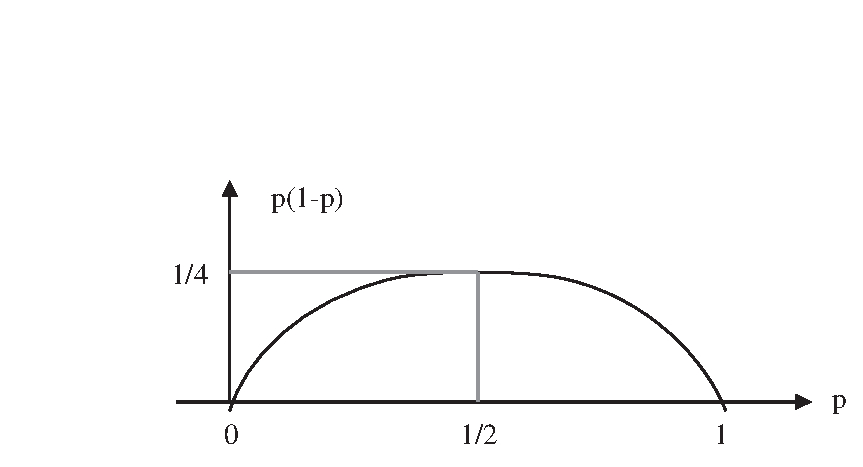
\includegraphics[scale=0.8]{figurer/fig7_4.pdf} 
 \caption{Funksjonen $p(1-p)$}
	\label{fig:p1p}
\end{figure}

Vi ser at $p(1-p)=1/4-{(p-1/2)}^2$, slik at funksjonen oppnår sin
største verdi 1/4 for $p=0.5$. Derfor er alltid $n\leq 1/(4{\Delta}^2)$.
 Velger vi antall observasjoner $n=1/(4{\Delta}^2)$,
 ser vi at vi er garantert det ønskede presisjonsnivå uansett
hva $p$ måtte være. Eksempelvis dersom vi ønsker $\Delta =0.01$,
får vi $n=1/(4{\Delta}^2)=2500$.

I mange situasjoner i praksis har en imidlertid en viss peiling
på størrelsen av $p$ på forhånd. Dersom vi, som i Eksempel
6, studerer antall defekte $X$ i en prøveproduksjon og vi vet fra
før at slik produksjon gir om lag 10\% defekte, er det rimelig å
velge $n$ ved å bruke formelen ovenfor med $p=0.10$. Dersom vi
ønsker $\Delta =0.01$ får vi $n=0.10(1-0.10)/0.01^2=900$, dvs.
betydelig lavere enn den ``pessimistiske'' $n$ ovenfor. Dersom
problemet iste\-den dreier seg om estimering av en kjønnsproporsjon,
f.eks. proporsjonen av hunkalver hos en bestemt kvegrase, og vi
vet at denne er nær $0.50$, er det klart at vi er nødt til å
velge $n$=2500 for å oppnå at $\Delta =0.01$.
\end{eksempel}

Dette eksemplet skulle klart vise betydning av å bruke $a$ priori
informasjon til å planlegge størrelsen av eksperimentet. Å ta
observasjoner koster både tid og penger. Vi ønsker ikke å gjøre
mer enn nødvendig for å oppnå en ønsket presisjon. På den
 annen side ønsker vi ikke å komme i den situasjon at hele
undersøkelsen viser seg å være verdiløs fordi vi i
utgangspunktet planla for få observasjoner. La oss se på nok et eksempel.\\

\begin{eksempel}{Hypergeometrisk situasjon}
Anta at $Y$ er hypergeometrisk fordelt $(N, M, n)$. vi ønsker å
estimere $a=M/N$ ved bruk av estimatoren $\hat{a} =Y/n$. Anta at vi
står fritt til å velge $n$ slik at estimatoren får et ønsket
standardavvik $\Delta$. Vi skal derfor ha (se Eksempel 5)

\[ var\hat{a}=\frac{N-n}{N-1} \cdot \frac{1}{n} \cdot a(1-a) =  {\Delta }^2 \]

\noindent Løser vi dette med hensyn på $n$ får vi

\[ n=\frac{a(1-a)}{\frac{a(1-a)}{N}+{\Delta}^2 \cdot \frac{N-1}{N}}
                                 \approx \frac{a(1-a)}{{\Delta }^2} \]

\noindent Tilnærmingen fås ved å la $N\rightarrow \infty $ i den
 eksakte formel, og gjelder derfor kun for stor $N$. Beregningen med den
tilnærmede formel er enklere, og gir en øvre skranke $n'$,
svarende til uendelig populasjon, for det nødvendige antall
obsevasjoner $n$. Det er lett å sjekke at $n$ kan (tilnærmet)
uttrykkes som

\[  n=n'\cdot \frac{1}{1+\frac{n'}{N}} \] 

\noindent Vi kan tolke brøken som en korreksjonsfaktor, som reduserer
det nødvendige antall observasjoner, som følge av at
populasjonen er endelig. For å få et inntrykk av
populasjonsstørrelsens rolle, ser vi på et regneeksempel der
 $n'=2500$, som bl.a. er tilfelle for $\Delta =0.01$ og $a=0.5$
(jfr. Eksempel 9). Vi får da

\begin{center}
\begin{tabular}{c|rrrrrc}
 $N$ & 100 & 1 000 & 10 000 & 100 000 & 1 000 000 & $\infty$ \\ \hline
 $n$ & 96 & 714 & 2 000 & 2 439 & 2 494 & 2 500
\end{tabular}
\end{center}

\noindent For små populasjoner vil $n$ utgjøre en betydelig andel av denne.
Ettersom populasjonen øker, vil $n$ ikke øke i samme takt, og når
populasjonen er stor, vil $n$ være en beskjeden andel av denne.
Heri ligger noe av grunnlaget for moderne meningsmålinger. I
Eksempel 7 der Lillevik hadde 10 000 stemmeberettigede, er det nødvendig
 med en stikkprøve på 2 000 for å oppnå et standardavvik
på 0.01 for estimert andel poltilhengere. I et land med 10
mill. stemmeberettigede, vil en landsomfattende meningsmåling
foran et presidentvalg med to kandidater høyst kreve en
stikkprøve på 2 500 for å oppnå samme presisjon.
\end{eksempel}


\section{Konfidensgrenser}

I mange situasjoner ønsker en å bruke observasjoner til å sette
grenser for verdien av ukjent modellparameter $\theta $. Dersom
det er knyttet en pålitelig\-hets\-garanti til beregning av grensene,
vil vi kalle dem {\em konfidensgrenser}. Vi taler om den nedre
konfidensgrense $\underline{\theta}$ og den øvre konfidensgrense
 $\overline{\theta}$ for
$\theta $, som sammen definerer et intervall 
$[\underline{\theta},\overline{\theta}]$.

\begin{center} \framebox[10cm]{\begin{minipage}{9cm}\rule{0cm}{0.5cm}
 \begin{definisjon}
Et {\em konfidensintervall} for en ukjent parameter $\theta$ er et
intervall med grenser som, med en gitt sannsynlighet $c$ kalt
{\em konfidensnivået}, omslutter $\theta$.
 \end{definisjon}
\end{minipage}} \end{center}

\noindent Det er opp til brukeren å velge
konfidensnivå, og dette er bl.a. bestemmende for lengden av
konfidensintervallet. Vi kan ønske oss et kort intervall (stor
presisjon) med høyt konfidensnivå (stor sikkerhet), men det er
klart at et lengre intervall kan garanteres med større sikkerhet
enn et kort. Et konfidensintervall kan oppfattes som mengden av
plausible parameterverdier i lys av den foreliggende informasjon.
Økes informasjonen vil en kunne ``skrelle vekk'' ytterligere
verdier, slik at en får et kortere intervall med den samme
sikkerhet. Et valgt kompromiss mellom krav til presisjon og
sikkerhet vil derfor kunne bestemme omfanget av observasjoner. I
forrige avsnitt ga vi en metode for tilnærmet beregning av
konfidensintervaller: I situasjoner der vi har en
forventningsrett estimator $\hat{\theta}$ for $\theta$ med kjent
standardavvik $\sigma (\hat{\theta})$, og med fordeling som kan
tilnærmes med normalkurven, vet vi at sannsynligheten for at 
$\hat{\theta}$ avviker fra den ukjente $\theta$ med høyst $k\cdot \sigma
(\hat{\theta})$, er tilnærmet lik arealet under normalkurven mellom $-k$
og $k$. Følgelig bestemmer

\[ \hat{\theta} \;\;\pm \;\; k \cdot \sigma (\hat{\theta}) \]

\noindent et konfidensintervall for $\theta$ med konfidensnivå $c$
tilnærmet lik $A(k)$, og tabellen i forrige avsnitt gir derfor 
tilnærmet $c$ for ulike valg av $k$, som kan oppfattes som en
sikkerhetsfaktor. I de fleste situasjoner er imidlertid $\sigma
(\hat{\theta})$ ukjent og må estimeres. Konfidensgarantien vil da bli
noe tvilsom.

Statistisk teori kan imidlertid anvise beregningsmåter for
konfidensgrenser med eksakt konfidensgaranti for mange aktuelle
modeller. Beregningsmåten er imidlertid spesifikk for den enkelte
modell og ofte nokså komplisert. Tabeller vil være et alternativ,
men blir ofte altfor omfangsrike når en skal dekke spekteret av
aktuelle konfidensnivåer og obser\-vasjons\-stør\-relser. For en del
aktuelle situasjoner, så som den binomiske og hypergeometriske,
vil beregning av eksakte konfidensgrenser kunne tilbys som del av
statistisk programvare. I Poissonsituasjonen er imidlertid
tabellene overkommelige, og i Tabell~\ref{tab:Konfidensgrenser_Poisson} 
i Appendiks~\ref{app:fordelngstabeller} gir vi
konfidensgrenser for forventningen i Poissonfordelingen for ulike
konfidensnivåer.\\


\begin{eksempel}{ Ulykkesrisiko}
La situasjonen være som i Eksempel 8, hvor vi ønsker et
konfidensintervall for forventet antall ulykker pr. år $\lambda$,
basert på observert antall et bestemt år $X$, som antas
Poissonfordelt. Dersom vi ønsker konfidensnivå lik 95\%, og
observerer $X=9$ ulykker, gir Tabell~\ref{tab:Konfidensgrenser_Poisson} eksakt nedre og øvre
konfidensgrense for $\lambda$ lik henholdsvis 4.12 og 17.08. Merk
at når disse grensene ikke ligger symmetrisk om estimatet 9,
skyldes det at Poissonfordelingen er skjev, mens
normaltilnærming gir de symmetriske grensene $9 \pm 6$. Hvis vi
kjenner det totale antall nordmenn $n$ under risiko, vil en kunne
dividere de funne tall med $n$, og få estimat og konfidensgrenser
for sannsynligheten for at en tilfeldig person under risiko
rammes i løpet av et år. Et forsikringsselskap med $m$ forsikrede
vil kunne multiplisere disse tall igjen med $m$, og få estimat og
konfidensgrenser for forventet antall utbetalinger i løpet av et
år.
\end{eksempel}

Tabell~\ref{tab:Konfidensgrenser_Poisson} har en rekke anvendelsesmuligheter: I binomiske
situasjoner der suksess-sannsynligheten $p$ er liten og $n$ er
stor, vet vi at antall suksesser $X$ er tilnærmet Poissonfordelt
med forventning $\lambda =n\cdot p$. Vi kan da få tilnærmede
konfidensgrenser for $p$ ut fra Tabell~\ref{tab:Konfidensgrenser_Poisson}, ved å dividere grensene
for $\lambda$ med $n$. Tilsvarende vil en i hypergeometriske
situasjoner der andelen spesielle $a=M/N$ er liten, og $n$ er
stor, men liten i forhold til $N$, ha at antall spesielle i
utvalget $Y$ er tilnærmet Poissonfordelt med forventning $\lambda
=n\cdot a=n\cdot M/N$. Vi kan da få tilnærmede konfidensgrenser
for $a$ ved å dividere grensene for $\lambda$ med $n$, samt
grenser for $M$ ved å multiplisere disse igjen med $N$. I slike
skjeve situasjoner gir Poissontilnærmingen langt mer pålitelige
grenser enn de som er basert på normaltilnærming, som imidlertid gir
best resultat i symmetriske situasjoner $(p\approx 0.5)$. Dersom
observerte antall er så stort at det ikke dekkes av Tabell~\ref{tab:Konfidensgrenser_Poisson}, vil
normaltilnærmingen likevel kunne gi tilfredstillende resultat.

I enkelte situasjoner er en bare interessert i den ene
konfidensgrensen. Det vil være tilfellet når en kun er opptatt av
hvorvidt den ukjente $\theta$ ikke er for høy, f.eks. under en
faregrense. Det er da nok å beregne en øvre konfidensgrense, slik
at vi har et ensidig konfidensintervall $( - \infty , \bar{\theta}]$.
Risikoen for at intervallet ikke fanger opp den ukjente $\theta$
er da bare knyttet til den øvre grensen, og vil typisk være
halvert i forhold til den tosidige risikoen $r=1-c$. Oppslag i
tabeller for tosidig konfidensnivå $c$ svarer derfor til et
ensidig konfidensnivå lik $c'=1-r/2=(1+c)/2$. I Eksempel 11 vil
15.71 være en øvre konfidensgrense for $\lambda$ med ensidig
konfidensnivå på 95\% (ved bruk av Tabell~\ref{tab:Konfidensgrenser_Poisson} og 90\% tosidig nivå).\\

\begin{eksempel}{Revisjon}
I forbindelse med vurdering av den interne kontroll hos en klient
gransker revisor utbetalinger mht. avvik fra avtalte kontroller
(signaturer etc.). En andel utbetalinger med kontrollavvik på 1\%
anses normalt, mens mer enn 5\% anses urovekkende. Revisor
gransker et tilfeldig utvalg på $n$=200 utbetalinger blant et mye
større antall registrerte utbetalinger, og observerer $Y$
utbetalinger med kontrollavvik. Siden $n$ er stor og andelen
utbetalinger med kontrollavvik $a$ er lite, er det rimelig å anta
at $Y$ er tilnærmet Poissonfordelt med forventning
$\lambda=n\cdot a$. La oss si at vi observerer $Y=4$, dvs. 2\% med
avvik i utvalget. Av Tabell~\ref{tab:Konfidensgrenser_Poisson} finner vi en øvre konfidensgrense
på 9.15 for $\lambda$ med konfidensnivå 95\%. Dette gir en øvre
grense lik 9.15/200=0.04525 for $a$, og revisor ser ingen grunn
til nærmere gransking. Merk imidlertid at dersom $a$ virkelig er
0.01, vil det være en betydelig risiko for at konfidensgrensen
faller over ``faregrensen'' på 0.05, som da krever nærmere
gransking. I følge Tabell~\ref{tab:Konfidensgrenser_Poisson} skjer 
det når $Y=5$ eller mer, som har sannsynlighet 0.0526 
(se Tabell~\ref{tab:Poisson_fordeling} med $\lambda = 200\cdot
0.01 = 2$). For å redusere denne risikoen må utvalget økes noe.
\end{eksempel}

\section{Hypotesetesting}

Mange statistiske undersøkelser tar sikte på å belyse fremsatte
hypoteser, og eventuelt klargjøre om hypotesene bør forkastes. Vi
vil fortsatt anta at vi har en delvis spesifisert modell for det
fenomen som studeres. Innenfor denne rammen vil en hypotese være
et utsagn om de ukjente elementene i modellen, dvs. som oftest
uspesifiserte modellparametre.

\begin{center} \framebox[10cm]{\begin{minipage}{9cm}\rule{0cm}{0.5cm}
 \begin{definisjon}
 En {\em hypotesetest} er en observasjonsbasert metode for å klargjøre
 om  en gitt hypotese vedrørende en statistisk modell, kalt 
{\em nullhypotesen} $H_0$, bør forkastes til fordel for en gitt
 {\em alternativ hypotese} $H_A$.
 \end{definisjon}
\end{minipage}} \end{center}

\noindent  $H_0$ og $H_A$ vil alltid utelukke hverandre gjensidig samt
utfylle alle muligheter som foreligger. Dette betyr at forkastning
av nullhypotesen $H_0$ medfører aksept av den alternative
hypotesen $H_A$. Oftest vil nullhypotesen være at vi
stiller oss reservert til en framsatt påstand, som da vil være
den alternative hypotesen.
Vi stiller oss imidlertid åpne for at observasjoner 
kan peke såpass i favør av den alternative hypotesen at vi velger
å gå inn for denne. Teorien for hypotesetesting tar sikte på
å etablere metoder som har innebygget visse garantier mot
feilslutninger.

\begin{center} \framebox[10cm]{\begin{minipage}{9cm}\rule{0cm}{0.5cm}
\begin{definisjon}
En {\em testmetode} er definert ved en stokastisk variabel $T$ avledet av
observasjonene, kalt {\em testobservatoren}, og et
 {\em forkastningsområde}, dvs. de verdier av $T$ som betyr at
 nullhypotesen $H_0$ skal forkastes. 
\end{definisjon}
\end{minipage}} \end{center}

\noindent Vi vil vanligvis kunne velge blant flere testmetoder, og
spørsmålet er da hvilke retningslinjer vi skal legge til grunn
for vårt valg. Vi vil her fokusere på risikoen for feilslutninger.

 To typer feilslutninger kan forekomme. På den ene
side kan vi komme til å forkaste $H_0$ når $H_0$ i virkeligheten
er riktig, dette kalles {\em forkastningsfeil}, mens vi på den
annen side kan komme til å la være å forkaste en hypotese som
burde ha vært forkastet, dette kalles {\em godtakingsfeil}.
De mulige situasjonene som kan oppstå er

\begin{center}
\begin{tabular}{|l|ll|} \hline 
                           & \multicolumn{2}{c|}{``Virkeligheten''} \\
Slutning                   & $H_0$ riktig & $H_A$ riktig \\ \hline
                   &                  &     \\
Ikke forkast $H_0$ & Korrekt slutning & Godtakingsfeil \\
                   &                  &       \\
Forkast $H_0$      & Forkastningsfeil & Korrekt slutning \\
                   &                  &               \\ \hline
\end{tabular}
\end{center}

\noindent I denne forbindelse innfører vi :
\begin{center} \framebox[10cm]{\begin{minipage}{9cm}
 \vspace{-0.6\belowdisplayskip}
\begin{eqnarray*}
 \alpha &=&\mbox{\ Sannsynligheten for forkastningsfeil ($\alpha$ -risiko)}\\
 \beta  &=&\mbox{\ Sannsynligheten for godtakingsfeil ($\beta$ -risiko)}
\end{eqnarray*} \mbox{}  \vspace{-0.7\belowdisplayskip}
\end{minipage}} \end{center}

\noindent Vi ønsker oss selvsagt en testmetode som innebærer at
 risikoen for begge typer feilslutninger er liten, men, som vi skal se, vil
disse to ønsker trekke i hver sin retning. I praksis må vi derfor
foreta en rimelig avveining mellom de to ønskene, eller alternativt
finne ut hvor omfattende undersøkelsen må være for at begge
risikoer er redusert til et akseptabelt nivå. Slike avveininger kan
gjøres ved hjelp av følgende begrep:
 
\begin{center} \framebox[10cm]{\begin{minipage}{9cm}\rule{0cm}{0.5cm}
\begin{definisjon}
{\em Styrkefunksjonen} til en test angående en parameter $\theta$ er
sannsynligheten for å forkaste $H_0$ betraktet som funksjon av
$\theta$, betegnet her med $\Pi (\theta )$. Dersom

\[\max_{\theta \in H_0}\Pi (\theta ) = \alpha \]
sier vi at testen har {\em signifikansnivå} $\alpha$, mens $\Pi (\theta )$
beregnet for en $\theta$ i $H_A$ kalles {\em styrken} i dette alternativet.
\end{definisjon}
\end{minipage}} \end{center}
Definisjonen av signifikansnivå innebærer at
$\Pi (\theta ) \leq \alpha $ for alle $\theta$ i nullhypotesen, med
likhet for minst en $\theta$, typisk for grensetilfellet mellom nullhypotese
og alternativ.

La oss illustrere de grunnleggende id\'{e}er omkring hypotesetesting
ved hjelp av et konstruert eksempel.\\

\begin{eksempel}{Testing i binomisk modell}
En mann påstår at han har evner til å forutsi utfallet av
myntkast. Han kan riktignok ikke spå riktig utfall hver gang, og en
rimelig tolking av påstanden vil være at hans sjanse for å spå
riktig utfall av et myntkast er større enn $\frac{1}{2}$,
som er sjansen for å spå riktig for en person uten slike evner,
og som er henvist til å velge sin ``spådom'' tilfeldig blant de
to mulighetene krone eller mynt. For å se om det er noen grunn
til å gi mannen rett i sin påstand, lar vi mannen få anledning
til å spå utfallet av et antall myntkast som utføres med en
rettferdig mynt. Det er rimelig å anta at sannsynligheten $p$ for
riktig spådom er den samme i hvert kast.
Anta  at vi stiller oss tvilende til mannens
påstand. Vi formulerer da den hypotese at mannen ikke er bedre
enn folk flest til å spå utfallet av myntkast, dvs. vår hypotese
er at $p=\frac{1}{2}$. Som vårt alternativ til hypotesen har vi at
mannen har spådomsevner, dvs. at $p >\frac{1}{2}$.
Anta at vi gir mannen anledning til $n$=10 myntkast. La $X$ være antall
riktige spådommer, og anta at de 10 spådommene representerer
uavhengige forsøk med hensyn til utfallene suksess og fiasko.
Vi kan da slutte at $X$ er binomisk fordelt $(n=10,p)$
der $p$ er ukjent. På grunnlag av
observert verdi av $X$ skal vi avgjøre om det er noen grunn til å
forkaste hypotesen, og følgelig måtte gi mannen rett.
Vi skal altså teste

\[ H_0 : p=\frac{1}{2} \mbox{\ \ mot \ \ } H_A : p> \frac{1}{2} \]

\noindent Mange riktige spådommer taler i favør av at
mannen har spådomsevner, og det er derfor rimelig å bruke $X$ som
testobservator og forkaste $H_0$ når $X$ er tilstrekkelig stor.
Vår testmetode blir derfor:

\[    \mbox{\ Forkast $H_0$ og påstå $H_A$ dersom $X\geq k$} \]

\noindent der $k$ er en passende valgt konstant. Problemet er å velge $k$
 slik at vi får en brukbar test. Forkastningsområdet vil i dette
eksemplet være alle mulige verdier av $X$ større enn eller lik $k$,
 som vi vil gi navnet testens {\em kritiske verdi}.

La oss først belyse risikoen for forkastningsfeil, dvs. påstå at
mannen har spådomsevner $(H_A)$ når han i virkeligheten ikke har
det $(H_0)$. Sannsynligheten for dette (signifikansnivået) blir

\[ \alpha = P_{H_0}(X\geq k) \]

\noindent der $P_{H_0}$ betegner sannsynlighet beregnet under forutsetning
av at $H_0$ er riktig. Av Tabell~\href{tab:Binomisk_fordeling_p05} over den binomiske fordeling
$(n=10, p=0.5)$ får vi

\begin{center}
\begin{tabular}{c|cccccc}
 $x$& $\cdots$ & 6 & 7 & 8 & 9 & 10 \\ \hline
 $P_{H_0}(X=x)$&$\cdots$&0.2051&0.1172&0.0439&0.0098&0.0010 
\end{tabular}
\end{center}
Av denne tabellen finner vi signifikansnivået $\alpha$ for
testen for ulike valg av den kritiske verdi $k$

\begin{center}
\begin{tabular}{c|cccccc}
 $k$& $\cdots$ & 6 & 7 & 8 & 9 & 10 \\ \hline
 $\alpha =P_{H_0}(X\geq k)$&$\cdots$&0.3770&0.1719&0.0547&0.0108&0.0010 
\end{tabular}
\end{center}

\noindent Dersom vi velger en metode som forkaster $H_0$ når $X\geq 8$
betyr det at sannsynligheten for å påstå spådomsevner når 
slike ikke er til stede blir ca. 5\%. Velger vi isteden å være litt mer
skeptiske og forkaste $H_0$ først når $X\geq 9$ blir denne
sannsynligheten redusert til ca. 1\%.
La oss så se på risikoen for godtakingsfeil, dvs. la være å
 påstå spådomsevner hos en mann som i virkeligheten har det.
Sannsynligheten for å la være å påstå $H_A$ når $H_A$
 er riktig skriver vi

\[ \beta=P_{H_A}(X < k). \]

\noindent Denne sannsynlighet vil avhenge av hvilken $p>0.5$ i alternativet
$H_A$ vi ser på. La oss interessere oss for alternativet $p=0.8$,
nedenfor kalt $H_1$. For den binomiske fordeling $(n=10, p=0.8)$
finner vi av Tabell~\ref{tab:Binomisk_fordeling}, for ulike valg av kritisk verdi $k$

\begin{center}
\begin{tabular}{c|cccccc}
 $k$& $\cdots$ & 6 & 7 & 8 & 9 & 10 \\ \hline
 $\beta =P_{H_1}(X < k)$&$\cdots$&0.0328&0.1209&0.3222&0.6242&0.8926 
\end{tabular}
\end{center}

\noindent Anta at vi insisterer på at sannsynligheten $\alpha$ for å
påstå spådomsevner når slike ikke er til stede skal være 
høyst ca. 0.05. Vi må da velge $k=8$ som kritisk verdi. Dette gir 
$\alpha =0.0547$. Vi ser imidlertid at dette valg medfører at såpass
gode spådomsevner som svarende til $p=0.8$ vil ha sannsynlighet på
hele $\beta = 0.3222$ for å ikke bli avslørt. Vår spåmann vil
kunne hevde at denne testen ikke vil gi ham en rimelig sjanse til
å vise sine ferdigheter. Vi ser imidlertid at dersom vi reduserer
$\beta$, f.eks. ved å isteden velge $k=7$ som kritisk verdi, vil
$\alpha$ måtte øke. Omvendt vil reduksjon av $\alpha$ medføre
økning av $\beta$. Med det gitte antall observasjoner, er det ikke
mulig å finne en testmetode som samtidig gjør $\alpha$ og $\beta$
liten. Dersom vi imidlertid foretar flere observasjoner, og
dermed får mer informasjon, vil trolig risikoen for
feilkonklusjoner kunne reduseres.
La oss forsøke med $n=30$ observasjoner. Nå blir $X$ binomisk
fordelt $(n=30, p)$. Av en større tabell over den binomiske
fordeling finner vi (alternativt: bruk normaltilnærming)

\[ P_{H_0}(X\geq 20)=0.0495 \mbox{\ \ \ \ \ } P_{H_1}(X < 20)=0.0257 \]

\noindent Med $n=30$ observasjoner og $k=20$ som kritisk verdi, får vi en
test som oppfyller kravet om at signifikansnivået $\alpha$
skal være høyst $0.05$ samtidig som $\beta$ er tilsvarende liten.
Vi har ovenfor vurdert testmetoden ut fra alternativet
$H_1$ $(p=0.8)$. De samme betraktninger kan gjøres gjeldende for et
vilkårlig annet valgt alternativ $p>0.5$.
Anta nå at vi har valgt å gjøre $n=30$ observasjoner og fastlagt
testmetoden til

\[   \mbox{Forkast $H_0$ og påstå $H_A$ når $X\geq 20$.} \]

\noindent Testmetodens egenskaper kan oppsummeres i styrkefunksjonen til
testen, som her er sannsynligheten
for å forkaste nullhypotesen betraktet som funksjon av $p$. Vi skriver

\[ \Pi (p)=P(X\geq 20). \]

\noindent Av en binomisk tabell finner vi for ulike $p$

\begin{center}
\begin{tabular}{c|cccccc}
 $p$& 0.5 & 0.6 & 0.7 & 0.8 & 0.9 & 1.0 \\ \hline
 $\Pi (p)$& 0.0495&0.2915&0.7304&0.9743&0.9999&1.0000 
\end{tabular}
\end{center}

\noindent $\Pi (p)$ angir testens evne til å avsløre at $p>0.5$ for de
ulike $p$ ($>0.5$). Vi sier at $\Pi (p)$ er testens styrke i
alternativet $p$ ($>0.5$). På Figur~\ref{fig:Styrkefunksjonen} finner vi igjen $\Pi (0.8)=1-
\beta$ og $\Pi(0.5)=\alpha$ (signifikansnivået).
\begin{figure}[ht]
\centering
\includegraphics[scale=0.8]{figurer/fig7_5.pdf}
\caption{Styrkefunksjonen for testen}
	\label{fig:Styrkefunksjonen}
\end{figure}
\end{eksempel}

Vi har her sett på situasjonen der nullhypotesen $p=p_0$ ble
testet mot alternativet $p>p_0$. I andre situasjoner vil $p<p_0$
være det aktuelle alternativ, se Eksempel 1. Dette gjøres på
tilsvarende måte, og beskrives ikke i detalj her, se Oppgave~31.
Forøvrig får problemet samme form som beskrevet ovenfor ved å
formulere hypotesen om $q=1-p$ isteden. I atter andre situasjoner
er det aktuelle alternativ $p\not= p_0$, som for eksempel når en
vil teste om en mynt er rettferdig ($p=1/2$ mot $p\not= 1/2$). I
dette tilfellet forkastes $H_0$ både når $X$ er stor og liten, se
Oppgave~32 for detaljer.\\

\noindent {\bf Merknad.} Mange foretrekker å formulere binomisk testing
med den standardiserte variable
\[ Z=\frac{X-np_0}{\sqrt{np_0(1-p_0)}} \]
som testobservator. Denne er tilnærmet standardnormalfordelt når
nullhypotesen er riktig, og $n$ er tilstrekkelig stor. \\

I praksis er en interessert i å planlegge antall observasjoner $n$ slik at
en har oppfylt en gitt $\alpha$-risiko og $\beta$-risiko. Det er brysomt å prøve
og feile  som i eksemplet, og en ferdig formel basert på
normaltilnærming er:
\[ n=(\frac{k_{\alpha}\cdot \sqrt{p_0(1-p_0)} + k_{\beta}\cdot
           \sqrt{p_1(1-p_1)}}{p_1-p_0})^2        \]
der $k_\alpha$ er punktet som har areal under normalkurven lik $\alpha$
til høyre for seg. Den kritiske verdi kan så beregnes ved
\[ k=np_0 \pm \frac{1}{2} \pm k_{\alpha} \cdot \sqrt{np_0(1-p_0)} \]
der en bruker minus eller plusstegnet alt ettersom alternativet til 
nullhypotesen går i negativ eller positiv retning.
I det tosidige tilfellet må en bruke $\alpha/2$ istedenfor $\alpha$  i
formelen og bruke to kritiske verdier (begge fortegnene).\\

\begin{eksempel}{Prosesskontroll}
Anta at vi studerer en løpende produksjonsprosess der den enkelte
artikkel kan enten klassifiseres som defekt eller intakt. Antar
vi at sannsynligheten $p$ for at en enkelt artikkel er defekt er
den samme for alle artikler samt at kvaliteten av artiklene er
uavhengig av hverandre, så er vi i en binomisk situasjon. Vi
antar at når prosessen er ''i kontroll'' så er av erfaring
defektsannsynligheten på et bestemt nivå $p_0=0.10$, og dersom
prosessen løper ut av kontroll så ytrer det seg kun ved at
defektsannsynligheten er økt, f.eks. innstiller seg på et nytt
nivå $p_1>p_0$. Dette kan skyldes maskinslitasje e.l. La oss
tenke oss at situasjonen er slik at ved arbeidsdagens slutt
undersøkes de $n$ sist produserte artiklene, antall defekte $X$
observeres og det avgjøres om det er grunn til å tro at prosessen
er ute av kontroll slik at maskinene bør justeres før
produksjonen tar til igjen neste morgen. Under de gitte
forutsetninger er $X$ binomisk fordelt $(n,p)$ der $p$ er ukjent.
Situasjonen kan formuleres som et hypotesetestingsproblem der
nullhypotese og alternativ er gitt ved
\begin{eqnarray*}
H_0: & p=p_0  & \mbox{ (prosessen er i kontroll)} \\
H_A: & p>p_0  & \mbox{ (prosessen er ute av kontroll).}
\end{eqnarray*}
Som testobservator brukes $X$ og vi
\begin{center}
forkaster $H_0$ og påstår $H_A$ dersom $X\geq k$\\
forkaster ikke $H_0$ dersom             $X<k$.
\end{center}
der $k$ er en passende valgt konstant. Forkastning og ikke-forkastning
vil her i praksis bety henholdsvis justering og ikke-justering av
produksjons\-prosessen. 
Anta at vi ønsker styrke 0.95 i alternativet $p_1=0.20$.
Problemstillingen er som ovenfor med $\alpha=0.05$ og $\beta=0.05$, slik at 
$k_{\alpha}=k_{\beta}=1.645$. Formelen ovenfor gir da $n=133$, som innsatt
gir $k=19.5$. Siden $k$ må være et heltall velger vi $k=20$.
Da blir $\alpha$ noe mindre enn $0.05$ på bekostning av $\beta$ som blir
 noe større enn $0.05$. Ved valg av $k=19$ blir forholdet omvendt.

I praksis blir statistisk prosesskontroll utført ved hjelp av
et såkalt kontrolldiagram, der data plottes regelmessig,
slik at verdifull informasjon som ligger i rekkefølgen
av observasjonene også kan blottlegges, mer om dette i Kapittel 15.
\end{eksempel}


Vi har i dette avsnittet diskutert
testing av hypoteser om sannsynligheter i binomiske situasjoner.
Framgangsmåten i forbindelse med testing av hypoteser om andeler
i hypergeometriske situasjoner er helt analog, og tas ikke opp
spesielt her.                                                       

La oss oppsummere og utdype noen av de innførte begreper:
Etter at en modell for vårt eksperiment er etablert og nullhypotese og
alternativ er fastlagt, står en overfor
valg av testobservator. I enkelte situasjoner er det opplagt hva
som bør velges (som i eksemplene ovenfor), i andre situasjoner kan
det foreligge flere muligheter. Anta at en testobservator $T$ er
valgt, en må da fastlegge forkastningsområdet, dvs. hvilke verdier
av $T$ (store, små eller både store og små) som bør bety
forkastning av nullhypotesen. Dette vil avhenge av
problemstillingen, dvs. hvilken alternativ hypotese som
foreligger. Ønsket om at testen skal ha et bestemt signifikansnivå
og styrke, er så bestemmende for antall observasjoner og testens kritiske
verdi.

Signifikansnivået $\alpha$ til en test angir
sannsynligheten for forkastningsfeil, dvs. å forkaste
nullhypotesen og dermed påstå den alternative hypotese når
nullhypotesen er riktig, mens $\beta =1-\Pi$, der $\Pi$ er styrken
 (styrkefunksjonen) til testen, angir sannsynligheten for godtakingsfeil,
 dvs. å la være å påstå den alternative hypotese
når denne er riktig.

Det må understrekes at de risikoer vi er villige til å tolerere må
komme til uttrykk på forhånd, før vi ser på observasjonene. 
Når vi så fastlegger testmetoden i henhold til våre ønsker, 
får vi en garanti på testmetodens pålitelighet. Eksempelvis kan
signifikansnivået $\alpha$ tolkes slik at ved gjentatt bruk av
samme metode i lignende situasjoner vil vi, gjennomsnittlig i det
lange løp, oppleve forkastningsfeil i $100\cdot \alpha \%$ av
tilfellene. Dersom testmetoden ikke er fastlagt på forhånd, er det
lett å la seg påvirke av observasjonene ved valg av metode. I
verste fall kan observatøren være forutinntatt i situasjonen,
og ved å titte på observasjonene kan han, ved å ''velge''
signifikansnivået tilstrekkelig stort (eller lite), oppnå den
konklusjon han ønsket seg. Dette er juks!

Når metoden er fastlagt kan vi ta fram observasjonene (eventuelt
innhente disse), finne den realiserte verdi av testobservatoren
 $T$, kall den $t$. Vi kan nå trekke vår konklusjon: forkastning av
nullhypotesen dersom $t$ er en verdi i det, på forhånd fastlagte,
forkastningsområdet. I motsatt fall konkluderer vi at de
foreliggende observasjoner ikke gir grunnlag for å forkaste
nullhypotesen.

Det at en nullhypotese er forkastet betyr ikke at vi har bevist,
i streng forstand, at nullhypotesen er feil. Heller ikke betyr
ikke-forkastning at vi har bevist at nullhypotesen er riktig.
Utsagn som ''det er statistisk bevist at ...'' bør alltid tas med
en klype salt. Som regel foreligger det en viss risiko for
feilkonklusjoner og disse bør gjøres kjent.


Det kan knyttes en forbindelse mellom bruken av
konfidensintervallet og hypotesetesting: Gitt en nullhypotese
angående en parameter $\theta$. Beregn et konfidensintervall for
$\theta$ med konfidensnivå $c$, ensidig eller tosidig alt
ettersom alternativet til nullhypotesen er det. Forkastes
nullhypotesen dersom denne ligger utenfor konfidensintervallet,
har vi en test med signifikansnivå $\alpha = 1 - c$.

Vi har ovenfor lagt vekt på å bruke teorirammen for
hypotesetesting til å diskutere de to typer feil i sammenheng.
Det virker både naturlig og nødvendig i beslutningssituasjoner
som kan gis en godta-forkast for\-mule\-ring. Slike problemer kan
også studeres i en videre beslutningsteoretisk ramme, der også
subjektiv kunnskap om ukjente parametre kan inngå. Dette aspekt
forfølges i Kapittel 16.

I resten av dette avsnittet skal vi
diskutere ulike sider ved hypotesetesting som objektivt
hjelpemiddel til å vurdere og formidle utsagnskraften i et
observasjonsmateriale, slik det ofte gjøres i utredninger og
vitenskapelige rapporter. På den ene side har vi tester som tar
sikte på å vurdere graden av tilpasning observasjonene har til
en bestemt modell, kalt {\em føyningstester}. Eksempler på
dette fins i Kapittel 7.7 og i Kapittel 9. På den annen side
har vi tester som angår et enkelt aspekt ved modellen. I mange
situasjoner dreier det seg om å teste nullhypotesen at det ikke
er noen sammenheng av et bestemt slag, ofte formulert som et
utsagn om en parameter, mot alternativet at sammenheng
foreligger. Testen skal gi grunnlag for å vurdere hvorvidt en
mulig observert sammenheng er {\em signifikant}, dvs. ikke kan
skyldes tilfeldigheter. Eksempler på dette fins i Kapittel 8, 10,
11 og 12.

I praksis ser en, nesten konvensjonelt, brukt
signifikanssnivåene 1\%, 2.5\% og 5\% (spesielt i vitenskapelige
anvendelser), og utfallet av en test rapporteres ofte slik ''det
observerte resultat er signifikant (evt. ikke signifikant) på 5\%
nivå''. Dette betyr at med signifikanssnivå 5\% vil
observasjonene medføre at nullhypotesen blir (evt.\ ikke blir)
forkastet. Noen har etablert den praksis å rapportere et resultat
som er signifikant på 5\% nivå, men ikke på 2.5\% nivå med *,
et resultat som er signifikant på 2.5\% nivå, men ikke på
1\% nivå med ** og
et resultat som er signifikant på 1\% nivå med ***. Mer vanlig er det
å rapportere resultatet av en test ved den såkalte $P$-verdien.

\begin{center} \framebox[10cm]{\begin{minipage}{9cm}\rule{0cm}{0.5cm}
\begin{definisjon}
Sannsynligheten for at testobservatoren skulle gi en verdi minst
like mye i favør av $H_A$ som det vi observerte, beregnet under
forutsetning av at $H_0$ er riktig, kalles {\em P-verdien} til
det observerte resultat.
\end{definisjon}
\end{minipage}} \end{center}

\noindent $P$-verdien gir en indikasjon på hvor utsagnskraftig det
observerte resultat er i favør av den alternative hypotesen, jo
mindre $P$-verdi desto mindre trolig er det at nullhypotesen er riktig.
Vi har følgende sammenheng mellom $P$-verdi og signifikansnivå: 

\begin{center} \framebox[10cm]{\begin{minipage}{9cm}
 \vspace{-0.6\belowdisplayskip}
\[ P\leq \alpha \Longleftrightarrow \mbox{\ \ $H_0$ forkastes ved
                               valgt signifikansnivå $\alpha$} \]
\mbox{}  \vspace{-0.7\belowdisplayskip}
\end{minipage}} \end{center}

\noindent Dette betyr at $P$ er det minste signifikansnivå som tillater at
hypotesen forkastes. Ved lesing av en  rapport med $P$-verdier, bør en 
på forhånd gjøre seg opp en mening om hvilken 
 risiko for forkastningsfeil en er villig til å løpe,
dvs. bestemme seg for $\alpha$.
Dersom den rapporterte $P$-verdi er mindre enn eller lik den valgte
$\alpha$, vil det si at det observerte resultat medfører
forkastning av nullhypotesen for vedkommende person.

La oss begrunne påstanden ovenfor i situasjonen der store verdier av
testobservatoren $T$ peker mot $H_A$, slik at vi forkaster $H_0$
når $T\geq k$, der $k$ er kritisk verdi. Med
signifikanssnivå $\alpha$ er $k$ bestemt ved at
 $\alpha = P_{H_0} (T\geq k)$. Hvis observert verdi av $T$ er $t$, blir
 $P$-verdien til det observerte resultat $ P=P_{H_0} (T\geq t) $, og vi ser at
 $t\geq k  \Leftrightarrow  P\leq \alpha$.
Tilsvarende begrunner vi resultatet dersom det er små
(eller både store og små) verdier av $T$ som peker mot $H_A$. \\

Til slutt noen kritiske kommentarer: Signifikanstesting blir ofte
utført som en bevisstløs pliktøvelse, med betydelig fare for å
villede seg selv og andre, bl.a. på grunn av ensidig
fokusering på forkastningsfeil, gjennom å tilpasse testen et
gitt signifikanssnivå eller beregning av $P$-verdi. De to
vanligste feilgrep er:\\
1. En betydningsfull sammenheng forblir
uoppdaget fordi rapportert ikke-signifikans skyldes
for få observasjoner, og dermed for liten teststyrke.\\
2. En rapportert signifikant sammenheng eller effekt oppfattes
feilaktig som betydningsfull. Selv den mest betydningsløse
forskjell fra nullhypotesen kan avsløres, dersom vi har mange nok
observasjoner.\\
 Begge feilgrep kan unngås ved å utføre
styrkebetraktninger, idet en da må ta stilling til hva som anses
for å være betydningsfulle forskjeller.

\section{Analyse av forskjeller}
Man ønsker ofte å sammenligne samme modellparameter $\theta$ i
to ulike si\-tua\-sjoner eller for to populasjoner
\begin{itemize}
\item  defektsannsynligheten $p$ ved to produksjonsmetoder
\item  andelen $a$ med et bestemt standpunkt i to populasjoner
\end{itemize}
La generelt ${\theta}_1$ og ${\theta}_2$ være parameteren for hver 
av de to situasjonene.  Vi kan da være interessert i å anslå
forskjellen ${\theta}_1 - {\theta}_2$ eller teste hypotesen at 
parametrene er like ${\theta}_1 = {\theta}_2$.  Anta at det foreligger 
uavhengige observasjoner fra hver av de to situasjonene/populasjonene.
Det er da klart at

\begin{center} \framebox[10cm]{\begin{minipage}{9cm}\rule{0cm}{0.5cm}
Med ${\hat{\theta}}_1$ og ${\hat{\theta}}_2$ uavhengige forventningsrette
estimatorer for hhv. ${\theta}_1$ og ${\theta}_2$ blir
\[ E({\hat{\theta}}_1-{\hat{\theta}}_2)={\theta}_1 - {\theta}_2 \mbox{\ ,\ \ } 
     \sigma ({\hat{\theta}}_1-{\hat{\theta}}_2)=
     \sqrt{{\sigma}^2({\hat{\theta}}_1)+{\sigma}^2({\hat{\theta}}_2)} \]
\mbox{}  \vspace{-0.7\belowdisplayskip}
\end{minipage}} \end{center}
Det betyr at ${\hat{\theta}}_1 - {\hat{\theta}}_2$ blir en 
forventningsrett estimator for ${\theta}_1 - {\theta}_2$ med 
standardavvik som kan beregnes ut fra standardavviket til hver av
estimatorene ${\hat{\theta}}_1$ og ${\hat{\theta}}_2$.
Dette standardavviket må i praksis oftest estimeres med 

\[  S({\hat{\theta}}_1-{\hat{\theta}}_2)=
       \sqrt{S^2({\hat{\theta}}_1)+S^2({\hat{\theta}}_2)} \]
der $S({\hat{\theta}}_1)$ og $S({\hat{\theta}}_2)$ er estimatorer for
hhv. $\sigma({\hat{\theta}}_1)$ og $\sigma({\hat{\theta}}_2)$.
I situasjoner av praktisk interesse, som binomiske og 
hypergeometriske situasjoner, vil fordelingen til 
${\hat{\theta}}_1 - {\hat{\theta}}_2$ etter standardisering kunne
tilnærmes med normalkurven.  Feilmarginer konstruert etter 
standardfeilmetoden kan derfor vurderes på vanlig tilnærmet 
måte, såfremt antall observasjoner ikke er for lite. \\

\begin{eksempel}{To produksjonsmetoder}
Anta at det produseres etter to metoder og man finner $X_1$ defekte
blant $n_1$ produserte etter metode 1, $X_2$ defekte blant $n_2$ 
produserte etter metode 2.  Antar vi at defektsannsynligheten ved
de to metodene er hhv. $p_1$ og $p_2$, er det rimelig å anta at
$X_1$ er binomisk fordelt $(n_1, p_1)$ og $X_2$ binomisk fordelt
$(n_2, p_2)$, samt at $X_1$ og $X_2$ er uavhengige.  Siden 
${\hat{p}}_1 = X_1/n_1$ og ${\hat{p}}_2 = X_2/n_2$ er 
forventningsrette estimatorer for hhv. $p_1$ og $p_2$ blir 

\[{\hat{p}}_1 - {\hat{p}}_2 \mbox{\ \ forventningsrett for\ \  } p_1 - p_2 \]
og standardavviket til denne estimatoren blir

\[ \sigma ({\hat{p}}_1-{\hat{p}}_2)=
          \sqrt{\frac{p_1(1-p_1)}{n_1}+\frac{p_2(1-p_2)}{n_2}} \]
som i praksis estimeres med $S({\hat{p}_1} - {\hat{p}}_2)$ definert 
ved at $p_1$ og $p_2$ erstattes med ${\hat{p}}_1$ og ${\hat{p}}_2$
i formelen ovenfor.  

Anta at det ble produsert $n_1 = n_2$ = 100 artikler med hver metode,
og at antall defekte ble henholdsvis $X_1$ = 9 og $X_2$ = 5.
Vi får da

\[  {\hat{p}}_1 - {\hat{p}}_2 = 0.09 - 0.05 = 0.04   \]
mens det tilhørende standardavvik anslås til 

\[ S({\hat{p}}_1-{\hat{p}}_2)= \sqrt{0.09\cdot 0.91/100+0.05\cdot
0.95/100}=0.036 \]
Det er derfor ingen grunn til å påstå at de to metodene 
generelt har ulik defektsannsynlighet.
\end{eksempel}

Hypergeometriske situasjoner der en ønsker å estimere 
forskjellen på andelene spesielle elementer i to populasjoner,
f.eks. andelen defekte i to produksjonspartier, ut fra tilfeldige 
utvalg, kan behandles på samme måte som i eksemplet.  Eneste
forskjell blir korreksjonsfaktorer for endelige po\-pula\-sjoner av typen
$(N-n)/(N-1)$, som kan utelates dersom utvalgene utgjør en liten 
andel av populasjonene.

I spørreskjemaundersøkelser trekkes ofte et utvalg fra en
større populasjon, mens en ved analysen av resultatene ofte bryter
ned på undergrupper, f. eks. kjønn, som ønskes
sammenlignet.  Antallet i hver gruppe er da ikke gitt på forhånd.
Likevel er det naturlig å rapportere standardavvik etter formlene
ovenfor.  Dette forutsetter at vi har et tilfeldig utvalg fra
populasjonen, som etter gruppering kan oppfattes som et tilfeldig
utvalg fra hver sin gruppe. \\

\begin{eksempel}{Spørreskjemaundersøkelse}
I en spørreskjemaundersøkelse ble $n$=400 tilfeldige personer
fra en populasjon spurt om deres holdning (ja/nei) til et bestemt
spørsmål.  Svarene ble gruppert på kjønn og resultatet ble
\begin{center}
\begin{tabular}{l|ll|l} 
         &         Ja       &     Nei        &      Sum     \\ \hline
Mann     &     95 (43.2\%)  &  125 (56.8\%)  &   220 (100\%) \\	
Kvinne   &     70 (38.9\%)  &  110 (61.1\%)  &   180 (100\%) \\ \hline
Sum      &    165           &  235           &   400         \\ \hline
\end{tabular}
\end{center}
Estimert Ja-forskjell mellom Mann - Kvinne 
\[         0.432 - 0.389 = 0.043   \]
Estimert standardavvik

\[\sqrt{0.432\cdot 0.568/220 + 0.389\cdot 0.611/180} = 0.049  \]
Her er antatt at populasjonen er så stor at korreksjonsfaktor for 
endelig populasjon er unødvendig. \\
\end{eksempel}
Vi er ofte interessert i å teste om det er forskjell mellom to
sannsynligheter

\[ H_0: p_1 = p_2 \mbox{\ \ \ mot \ \ \ } H_A: p_1 \neq p_2 
                       \mbox{\ \ ( evt. $>$ eller $<$ )}  \]
En mulig testobservator er 
\[   U=\frac{\hat{p}_1-\hat{p}_2}
           {\sqrt{(\frac{1}{n_1}+\frac{1}{n_2})\hat{p} (1-\hat{p} )}} \]
der ${\hat{p}} = (X_1 + X_2)/(n_1 + n_2)$, dvs. at nevneren er en estimator
for $\sigma({\hat{p}}_1 - {\hat{p}}_2)$ som forutsetter at $p_1=p_2$.
Det kan vises at når $H_0$ er riktig, så kan fordelingen til $U$
tilnærmes med normalkurven, slik at kritiske verdier eller P-verdier for
testen kan beregnes tilnærmet.

Med dataene i Eksempel 15 blir $U=1.63$, som gir $P=0.102$ for tosidig
alternativ og $P=0.051$ for ensidig alternativ.

U-testen er forøvrig likeverdig med den såkalte
kjikvadrattesten for uavhengighet i 2 $\times$ 2-tabell presentert i
Kapittel 9. En alternativ test er Fisher-Irwins test beskrevet i Kapittel 10.


\section{En test for realisme av en modell.}

I Kapittel 1 introduserte vi begrepet sannsynlighetsmodell, og ønsket at
slike skulle forklare empiriske fenomener. Vi har i dette kapitlet sett 
hvordan vi kan teste utsagn om enkeltsannsynligheter basert på data.
Vi skal nå se hvordan vi kan teste om en gitt modell er realistisk.\\


\begin{eksempel}{Rettferdig terning?}
En modell for en rettferdig terning er
\begin{center}
\begin{tabular}{lrrrrrr}
Utfall ($u_i$):   & 1 & 2 & 3 & 4 & 5 & 6 \\
Sannsynligheter ($p_i$):&$\frac{1}{6}$&$\frac{1}{6}$&$\frac{1}{6}$
                        &$\frac{1}{6}$&$\frac{1}{6}$&$\frac{1}{6}$
\end{tabular}
\end{center}
Vi har en vanlig terning og ønsker å teste om den er rettferdig.
For dette formål ble terningen kastet $n=240$ ganger og vi
observerte antall ganger terningen viste henholdsvis $1,2,...,6$
øyne. Vi fikk
\begin{center}
\begin{tabular}{lrrrrrr}
Utfall ($u_i$):   & 1 & 2 & 3 & 4 & 5 & 6 \\
Hyppighet ($X_i$):&32 &44 &36 &45 &34 &49
\end{tabular}
\end{center}
Forventet antall kast med $i$ øyne, dersom terningen er rettferdig,
blir $EX_i=np_i=240\cdot 1/6=40$. Er de observerte antall forenlig med dette,
eller så avvikende at modellen bør forkastes?
Vi trenger en testobservator som sammenfatter graden av avvik.
\end{eksempel}


La oss diskutere problemstillingen i generelle vendinger:
Gitt et eksperiment med et endelig antall utfall hvor det
foreligger en sannsynlighetsmodell med utfall og sannsynligheter
gitt ved
\begin{center}
\begin{tabular}{cccccccc}
   & & $u_1$ & $u_2$ & $u_3$ & $\ldots $ & $u_m$ & \\
 $H$: & & $p_1$ & $p_2$ & $p_3$ & $\ldots $ & $p_m$ & $(\sum_{i=1}^m p_i=1)$. 
\end{tabular}
\end{center}
Det råder tvil om modellen er realistisk og den er foreløpig satt
opp som en arbeidshypotese H. For å få et inntrykk av om modellen
er realistisk, utføres eksperimentet $n$ ganger uavhengig av
hverandre og under de samme betingelser. La $X_1, X_2, \ldots, X_m$
være antall ganger vi observerer henholdsvis $u_1, u_2, \ldots , u_m$
 $(\sum_{i=1}^m X_i=n)$.

Under de gitte forutsetninger og modell $H$, ser vi at $X_i$ er
binomisk fordelt $(n,p_i)$ for $i=1, 2, \ldots , m$.  Dette innses ved å betrakte
$u_i$ som suksess; vi har da $n$ binomiske forsøk med
suksessannsynlighet $p_i$. Følgelig er $EX_i=np_i$ og $varX_i=np_i(1-p_i)$.
Et egnet mål på hvor godt observasjonene i det store og hele
samsvarer med modellen er
\[ Q=\sum_{i=1}^{m}\frac{{(X_i-np_i)}^2}{np_i} \]
Dersom modellen er realistisk vil $X_i$ være forholdsvis nær sin
forventning $np_i$, i hvert fall gjennomgående nærmere enn når
modellen er urealistisk. En stor verdi på $Q$ vil derfor indikere
at modellen ikke er realistisk, spørsmålet er bare hvor stor $Q$
må være for at en slik tvil om at modellen er realistisk synes
berettiget
\footnote{I uttrykket for $Q$ har vi i hvert ledd
dividert med forventningen $np_i$, bl.a. fordi et gitt avvik
$X_i-np_i$ bør tillegges mer vekt når $np_i$ er liten enn når
$np_i$ er stor.}.
 La oss beregne forventningen til $Q$ ut fra
forutsetningene ovenfor

\begin{eqnarray*}
 EQ&=&\sum_{i=1}^{m}\frac{1}{np_i}E{(X_i-np_i)}^2=
                           \sum_{i=1}^{m}\frac{1}{np_i}varX_i \\
   &=&\sum_{i=1}^{m}\frac{1}{np_i}np_i(1-p_i)=\sum_{i=1}^{m}(1-p_i)=m-1
\end{eqnarray*}
Det kommer derfor neppe på tale om å så tvil om modellen er
realistisk før $Q$ er noe større enn $m-1$.

Anta at observasjonene er slik at den beregnede verdi av $Q$ er
tallet $q$. Vi ønsker et mål på hvor oppsiktsvekkende det
observerte resultat er i lys av modellen. Et slikt mål vil være

\[ P=P_H(Q\geq q) \]
beregnet på grunnlag av modellen $H$. $P$ er altså
sannsynligheten, med den gitte modell, for å få det observerte
resultat eller et resultat som taler enda mer i disfavør av
modellen. Dersom denne $P$-verdi er liten, er det observerte
resultat overraskende og det kan indikere at modellen $H$ er
urealistisk. Hvor liten $P$-verdi som skal til for at vi forkaster
denne modellen, er vårt eget valg, og vil avhenge av
omstendighetene, bl.a. den bruk vi hadde tenkt å gjøre av
modellen.

For å beregne $P$-verdien trenger vi altså å kjenne
sannsynlighetsfordelingen til $Q$ under forutsetningene ovenfor.
Den eksakte fordeling er generelt vanskelig å etablere, vi må
nøye oss med følgende tilnærmelse. \footnote{Denne tilnærmelsen
tilskrives Karl Pearson (1857-1936), som var en av pionerene i
moderne statistisk teori.}

\begin{center} \framebox[10cm]{\begin{minipage}{9cm}\rule{0cm}{0.5cm}
{\bf Kjikvadrattilnærmelsen:} Sannsynlighetsfordelingen (histogrammet)
 til $Q$ vil, under forutsetning av at modellen $H$ gjelder, når $n$
vokser, nærme seg en kontinuerlig kurve, kalt
{\em kjikvadratkurven} med $m-1$ frihetsgrader.
 \footnote{Av historiske årsaker: $m-1$ er antall frie parametre;
 når $m-1$ $p_i$'er er gitt, er også den siste bestemt.}
\end{minipage}} \end{center}

\noindent Det matematiske uttrykk for kurven utelates her. Vi nøyer oss med
å fastslå at kurven ikke avhenger av sannsynlighetene $p_1, p_2,
..., p_m$ i modellen, men bare avhenger av antall utfall $m$.
Kurvens tyngdepunkt vil forskyves mot høyre for økende $m$, som
synes rimelig ettersom $EQ=m-1$.

\begin{figure}[ht]
\centering
   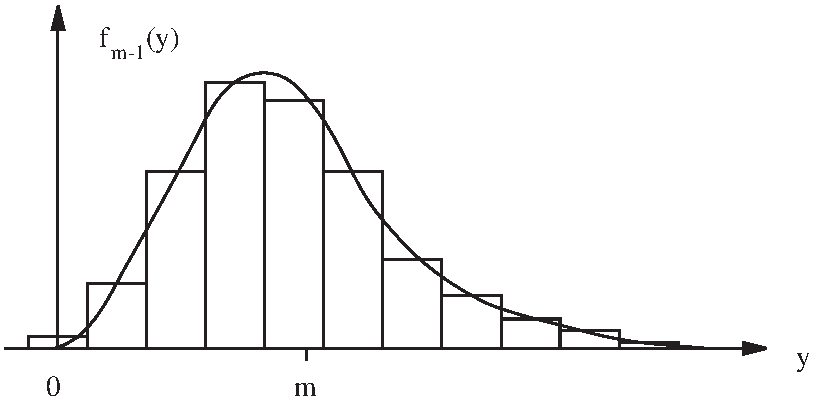
\includegraphics[scale=0.8]{figurer/fig7_6.pdf} 
 \caption{Kjikvadrattilnærmelsen}
	\label{fig:X2approx}
\end{figure}

\noindent I Figur~\ref{fig:X2approx} har vi inntegnet et tenkt histogram for $Q$ og
tilhørende kji\-kvadratkurve. Lar vi $ \bar{F}_{m-1}(q)$ betegne
arealet til høyre for $q$ under kji\-kvadratkurven med $m-1$
frihetsgrader, vil derfor for store $n$

\[ P_H(Q\geq q)\approx  \bar{F}_{m-1}(q). \]
For å kunne bruke dette resultatet i praksis trenger vi å ha
tabellert $\bar{F}_{\nu}(q)$ for ulike $q$ og ulike frihetsgradtall
 $\nu$ . En slik tabell er Tabell~\ref{tab:Kjikvadrat_Areal} i Appendiks~\ref{app:fordelngstabeller}. Vi kunne
alternativt ha tabellert  $F_{\nu}(q)$  som er arealet til venstre
for $q$. Da er  $\bar{F}_{\nu}(q)=1- F_{\nu}(q)$, men i forbindelse med
kjikvadratkurver trenger en i praksis oftest de høyresidige
arealene. Merk at siden kji\-kvadratkurver må tabelleres for en
rekke frihetsgradtall $\nu = 1,2,3,\ldots$, kan hver tabell
nødvendigvis ikke være så omfattende som tilfellet var med
normalkurven. For frihetsgradtall større enn 5 har vi måttet nøye
oss med såkalte fraktiltabeller, dvs. angi de punkter $q$ som har
bestemte arealer til høyre for seg (Tabell~\ref{tab:Kjikvadrat_Fraktiler}).
For kjikvadrattilnærmelsen vil graden av tilnærming avhenge av
$n$ og til en viss grad av $p_i$'ene i modellen, en ser ofte
anbefalt at tilnærmelsen er brukbar for de fleste praktiske
formål dersom $np_1, np_2, \ldots , np_m$ alle er større enn 5, men
også i situasjoner hvor dette ikke er tilfelle vil tilnærmelsen
gi en pekepinn på størrelsesorden av sannsynlighetene. \\

\addtocounter{eksecount}{-1}
\begin{eksempel}{Rettferdig terning? (fortsatt)}
Med de data som er gitt ovenfor beregner vi testobservatoren

\[ Q=\sum_{i=1}^{m}\frac{{(X_i-np_i)}^2}{np_i} =
          \sum_{i=1}^{6}\frac{{(X_i-40)}^2}{40}=5.95 \] 
Dersom terningen er rettferdig, er $EQ=5$ og det observerte
resultat er ikke særlig mye større enn dette. Under denne
forutsetningen kan sannsynlighetsfordelingen til $Q$ tilnærmes
med kjikvadratkurven med $6-1=5$ frihetsgrader. 
Ifølge Tabell~\ref{tab:Kjikvadrat_Areal} blir $P(Q\geq 5.95)\approx 0.31$, dvs. sannsynligheten for å
observere et resultat som det gitte, eller et som er enda mer
avvikende fra ''det forventede'' $40,40,\ldots ,40$ målt med $Q$, er
ca. lik 0.31. Det observerte resultat kan derfor ikke sies å
være tilstrekkelig oppsikts\-vekkende til at det gir grunnlag for å
påstå at terningen er falsk.\\
\end{eksempel}

\begin{eksempel}{Reklamasjoner}
Et varemagasin har erfart at siste år kom det gjennomsnittlig en
reklamasjon pr. åpningsdag. Man ønsker å teste om det er rimelig
å anta at antall reklamasjoner på en gitt dag er Poissonfordelt
med forventning 1. For dette formål noteres antall reklamasjoner
hver dag i en periode på $n=50$ åpningsdager. Alle opplysninger
som trengs er gitt i tabellen

\begin{center}
\begin{tabular}{rlrcr}
 $u_i$&            & $X_i$ & $p_i$ & $np_i$ \\ \hline
   0  &            &   15  & 0.368 &  18.4  \\
   1  &            &   21  & 0.368 &  18.4  \\
   2  &            &   12  & 0.184 &   9.2  \\
   3  &            &    2  & 0.061 &   3.0  \\
   4  & eller flere&    0  & 0.019 &   1.0  \\ \hline
\end{tabular}
\end{center}
Utfallene $u_i (i=1,2,\ldots ,5)$ representerer de ulike antall
reklamasjoner som kan inntreffe i løpet av en dag, der vi har
gruppert sammen 4 eller flere for å få et endelig og
rimelig antall grupper. $X_i$'ene er antall dager som vi
observerte de ulike utfall. De forventede antall dager dersom
Poisson\-modellen holder er $np_i$, der de teoretiske
Poissonsannsynlighetene $p_i$ er hentet fra Tabell~\ref{tab:Poisson_fordeling}. I dette
tilfellet blir

\[ Q=\sum_{i=1}^{5}\frac{{(X_i-np_i)}^2}{np_i} =3.18 \]
Dersom Poissonmodellen benyttes vil $EQ=4$. Her er observert $Q$
noe mindre og det observerte resultat gir derfor intet grunnlag
for å vrake Poissonmodellen. Her kan fordelingen til $Q$
tilnærmes med kjikvadratkurven med $5-1=4$ frihetsgrader og
sannsynligheter for det gitte resultat eller et mer avvikende vil
faktisk være mer enn 50\% når Poissonmodellen benyttes.

Det er også mulig å teste om en Poissonmodell er realistisk uten antatt
forventning. Denne må i så fall
estimeres ut fra dataene ved gjennomsnittet. Framgangsmåten ved testingen
er ellers den samme, men frihetsgradtallet er en mindre. \\
\end{eksempel}


I de to eksemplene ovenfor ga det observerte tallmateriale ingen
grunn til å vrake den oppsatte modell. Vi kunne ønske oss et mer
omfattende materiale for å etterprøve modellene, og det kan ikke
utelukkes at dette vil kunne føre til at modellene vrakes på et
senere tidspunkt. En må imidlertid være klar over at i mange
situasjoner vil en modell være brukbar for sitt formål selv om
den er noe grov. Et meget stort tallmateriale vil derfor lett
kunne gi forkastning av en grov modell også når denne avviker
ubetydelig, for praktiske formål, fra en mer realistisk modell.
Dette er ikke ment som en advarsel mot å samle inn ytterligere
materiale for å etterprøve modeller,
snarere tvert imot. Man bør bare være bevisst hvilket formål
modellen skal tjene og selv foreta rimelige avveininger med
hensyn til realisme og brukbarhet av den oppsatte modell, jfr. de
betraktninger som ble gjort i Kapittel 1. \\

\small
 $\star$Med den terminologi vi har innført ovenfor vil generelt $X_1,
X_2, \ldots, X_m$ være multinomisk fordelt med parametre $(n,
p_1, p_2, \ldots , p_m)$ se Kapittel 6.8, og problemstillingen er å
teste en hypotese $H$ om disse parametrene. Som testobservator
brukes $Q$ og testmetoden består i at hypotesen forkastes når
$Q\geq k$, der $k$ er en passende valgt konstant. Ønskes
signifikansnivå $\alpha$ må $k$ velges slik at $P_H(Q\geq k) = \alpha$.
 For øvrig vil forkastning være ekvivalent
med at $P$-verdien er mindre enn $\alpha$. Med dette kan vi altså
fastlegge sjansen for å forkaste hypotesen (modellen) når denne
er riktig (realistisk). På den annen side ønsker vi å studere
sjansen for å la være å forkaste en hypotese som er feil (modell
som åpenbart er urealistisk). Med andre ord ønsker vi studere
styrkefunksjonen til testen. Dette er et relativt komplisert
problem, bl. a. fordi en slik funksjon vil avhenge av alle
$p_1, p_2,\ldots ,p_m$, og vi kan ikke
gå inn på det her. Vi skal imidlertid ikke underslå at det finnes
andre testmetoder som er velegnet dersom man har spesielle
alternativer til hypotesen i tankene. Kjikvadrattesten som vi har
presentert ovenfor er imidlertid relativt enkel å utføre og
benyttes ofte i praksis.

Den problemstilling som er presentert i dette avsnittet svaret
til å teste en helspesifisert hypotese om parametrene i en
multinomisk modell. Problemstillingen kan utvides til å teste
delvis spesifiserte hypoteser i denne modellen. Dette kan bl.a.
brukes til å teste om observasjoner er forenlig med en bestemt
forde\-lingstype, og ved analyse av krysstabellerte kategoridata 
(se Kapittel 9), som er ofte forekommer ved meningsmålinger og
markedsundersøkelser.
\normalsize

\section{Oppgaver}
\small
\begin{enumerate}
\item I en binomisk situasjon med suksessannsynlighet $p$
    observeres antall suksesser $X$ i løpet av $n$ forsøk.
\begin{itemize}
\item[(a)] Finn en forventningsrett estimator for
   fiaskosannsynligheten $q=1-p$, og beregn dennes varians.
 
\item[(b)] Finn en forventningsrett estimator for forskjellen
            $r=q-p=1-2p$, og beregn dennes varians.
\end{itemize}

\item I en hypergeometrisk situasjon der antall spesielle
elementer i populasjonen er $M$, observeres antall spesielle
elementer $Y$ i et utvalg på $n$ elementer.
\begin{itemize}
\item[(a)] Finn en forventningsrett estimator for $M$ og angi dens
   varians.
\item[(b)] Finn en forventningsrett estimator for antall vanlige elementer i populasjonen $N-M$ og angi dens varians.
\end{itemize}

\item La $X$ være antall suksesser i løpet av $n$ binomiske
forsøk. Som estimator for suksessannsynligheten $p$ brukes
$\hat p=X/n$. Finn $P(\mid\hat p-p\mid\leq 0.1)$ i følgende
situasjoner
\begin{center}
\begin{tabular}{rrccl}
(a)& $p=0.5$ & og & $n=5$, 10, 25, 50, 100 \\
(b)& $p=0.4$ & og & $n=5$, 10, 25, 50, 100 \\
(c)& $p=0.2$ & og & $n=5$, 10, 25, 50, 100.
\end{tabular}
\end{center}
Bruk normaltilnærming i situasjoner der binomiske tabeller ikke rekker.
\item
\begin{itemize}
\item[(a)] Ta for deg et kronestykke, og knips den $n$ ganger.
   Estimer sannsynligheten for kron $p$ og oppgi
    feilmarginer dersom (i) $n=10$   (ii) $n=100$.
\item[(b)] Ta for deg en tegnestift, og kast den $n$ ganger.
    Estimer sannsynligheten for at den faller med spissen i
    været $p$ og oppgi feilmarginer dersom (i) $n=10$  (ii) $n=100$.
\item[(c)] Ta for deg en terning, og kast den $n$ ganger. Estimer
   sannsynligheten for å få sekser $p$ og oppgi
    feilmarginer dersom (i) $n=10$  (ii) $n=100$.
\end{itemize}

\item Finn fram en pose erter og tell opp et visst antall, f. eks.
$N=100$. La en venn merke en del av ertene før alle legges i
en boks, uten at du får vite hvor mange som er merket.
Forsøk så å anslå andelen og antallet merkede erter ut fra
et utvalg på $n=10$ erter. Gjenta eksperimentet med et annet
blandingsforhold. Forsøk også andre stikkprøvestørrelser,
f.eks. $n=25$. Vurder i hvert tilfelle risikoen for
estimeringsfeil. Er det mulig å besvare spørsmålene dersom
du heller ikke vet antallet kuler i boksen?

\item Betrakt populasjonen av $N=216$ studenter i Eksempel 1.7.
Estimer på grunnlag av en stikkprøve andelen studenter \\
(i)  med mindre enn 10 kroner på seg,\\
(ii) med mer enn 100 kroner på seg. \\
Vurder påliteligheten av estimatet.
Forsøk ulike stikkprøvestørrelser, f. eks. $n=10$ og $n=25$.
Angående trekningsmåten, se Oppgave~\ref*{kap:introduksjon}.9.

\item To estimatorer $\hat{\theta}$ og $\check{\theta}$ for en parameter
$\theta$ er foreslått. Hvilken vil du velge dersom deres
sannsynlighetsfordelinger er henholdsvis
\begin{center}
\begin{tabular}{c|ccccc}
 $k$ & $\theta -2$ &$\theta -1$ &$\theta$ &$\theta +1$ &$\theta +2$ \\ \hline
 $P(\hat{\theta}=k)$& 0.1 & 0.2 & 0.4 & 0.2 & 0.1 \\                       
 $P(\check{\theta}=k)$& 0.2 & 0.0 & 0.6 & 0.0 & 0.2
\end{tabular}
\end{center}

\item Anta $X_1$ og $X_2$ forventningsrette estimatorer for
henholdsvis $\theta _1$ og $\theta _2$.
\begin{itemize}
\item[(a)] Lag med utgangspunkt i $X_1$ og $X_2$ forventningsrette
estimatorer for \\
(i)   $\theta _1 + \theta _2$ \ \
(ii)  $\theta _1 - \theta _2$ \ \
(iii) $(\theta _1 + \theta _2)/2$.
\end{itemize}
Anta at $X_1$ og $X_2$ er uavhengige med samme varians $\sigma ^2$.
\begin{itemize}
\item[(b)] Finn variansen til estimatorene i (a).
\end{itemize}

\item Anta at $X_1$ og $X_2$ er stokastiske variable med forventninger\\
$EX_1=\theta_1 + \theta_2$ og $EX_2=\theta_1 - \theta_2$.
\begin{itemize}
\item[(a)] Lag med utgangspunkt i $X_1$ og $X_2$ forventningsrette
     estimatorer for $\theta_1$ og $\theta_2$.
\end{itemize}
Anta at $X_1$ og $X_2$ er uavhengige med samme varians $\sigma^2$.
\begin{itemize}
\item[(b)] Finn variansen til estimatorene i (a).
\end{itemize}

\item La $\hat{\theta}$ være en forventningsrett estimator for $\theta$
med fordeling som kan tilnærmes med normalkurven.
\begin{itemize}
\item[(a)] Dersom $\sigma (\hat{\theta})$ er $0.6$, finn tilnærmet
$P(\mid \hat{\theta} - {\theta} \mid \leq 0.4)$.
\item[(b)] Dersom $\sigma (\hat{\theta})$ er $0.8$, finn $d$ slik at
$P(\mid \hat{\theta} - \theta \mid \leq d) \approx 0.85$.
\item[(c)] Dersom vi krever $P(\mid \hat{\theta} - \theta \mid \leq
0.7)\geq 0.80$, hvor liten må standardavviket til
$\hat{\theta}$ i så fall være.
\end{itemize}

\item En bedrift masseproduserer en artikkel. Ut fra erfaring fra
de senere ukers produksjon antar man at
defektsannsynligheten er $p_0$. Det utføres så en overhaling
av produksjonsutstyret, og etter denne antas
defektsannsynligheten å være $p$ (mindre enn $p_0$); $p$
ønskes estimert.
\begin{itemize}
\item[(a)] Hvor mange artikler $n$ må minst undersøkes for at
    standardavviket til estimatoren skal bli høyst $0.01$ dersom\\
(i) $p_0=0.05$ \ \ \    (ii) $p_0=0.10$ \ \ \    (iii) $p_0=0.15$.
\item[(b)] Finn i hvert av disse situasjonene tilnærmet
       sannsynligheten for at estimatoren skal avvike høyst
        $0.015$ enheter fra den korrekte $p$.
\end{itemize}

\item En bedrift masseproduserer artikler. Man har erfart at
defektprodusenten vanligvis ikke overstiger $a_o$. En dag er
det produsert $N$ artikler, hvorav antall defekte $M$ er
ukjent. Man ønsker å estimere brøkdelen $a=M/N$ av defekte
artikler på grunnlag av et tilfeldig utvalg fra dagsproduksjonen.
\begin{itemize}
\item[(a)] Hvor mange artikler $n$ er det rimelig å velge ut
dersom en ønsker en estimator med standardavvik høyst
lik $0.01$ i tilfellene
\begin{center}
\begin{tabular}{rll}
(i)  &  $N=100$  &  $a_0=0.05$, 0.10, 0.15\\
(ii) &  $N=500$  &  $a_0=0.05$, 0.10, 0.15\\
(iii)&  $N=1000$ &   $a_0=0.05$, 0.10, 0.15\\
(iv) &  $N=10000$ &  $a_0=0.05$, 0.10, 0.15
\end{tabular}
\end{center}
\item[(b)] Finn i hvert av disse tilfellene tilnærmet
   sannsynligheten for estimatoren skal avvike høyst
   $0.015$ enheter fra den korrekte $a$.
\end{itemize}

\item  Forskjellen i defektsannsynlighet med to produksjonsmetoder 
$p_1 - p_2$ ønskes anslått ut fra andelen defekte blant henholdsvis
 $n_1$ og $n_2$ produserte artikler etter de to metodene.
\begin{itemize}
\item[(a)] Finn standardavviket til estimatoren i tilfellet at $p_1=p_2=p$
\item[(b)] Finn tilnærmet sannsynligheten for at estimatoren gir
verdi mellom $-0.1$ og $0.1$ dersom $n_1=n_2=20$ og \\
(i) $p_1=p_2=0.5$  \ \ \   (ii) $p_1=p_2=0.3$. \\
Hint: Bruk normaltilnærmelse, jfr. Kapittel 7.6..
\item[(c)] Hvor mange artikler av hvert slag må produseres for at 
standardavviket skal bli høyst 0.05?
\end{itemize}

\item Vis formelen

 \[E(\hat{\theta} - \theta)^2=var\hat{\theta}+(E\hat{\theta}-\theta)^2 \]
Hint: Skriv ${(\hat{\theta} - \theta)}^2={(\hat{\theta} -
E\hat{\theta} + E\hat{\theta} - \theta)}^2$ og kvadrer ut.

\item La $X$ være binomisk fordelt $(n,p)$. Som estimator for $p$
er foreslått $\tilde{p} =(X+1)/(n+2)$. Vis at
\begin{itemize}
\item[(a)]  $E\tilde{p}=p+\frac{1-2p}{n+2} $
\item[(b)]  $E{(\tilde{p}-p)}^2=\frac{1}{{(n+2)}^2}(np(1-p)+{(1-2p)}^2) $
\end{itemize}
Sammenlign denne estimatoren med den vanlige $\hat{p} =X/n$
når $n=5$ og når $n=50$ (Tegn figur!).

\item La $X$ være binomisk fordelt $(n,p)$. En estimator for $p$
er $p_0 = \frac{1}{2}$, dvs. det observerte resultat blir
neglisjert og $\frac{1}{2}$ oppgis som estimat uansett.
Sammenlign denne estimator med $\hat{p} =X/n$ og $\tilde{p}=(X+1)/(n+2)$.

\item En bedrift består av to avdelinger. Man ønsker å estimere
sannsynligheten for at en vilkårlig valgt arbeider utsettes
for en viss type arbeidsuhell i løpet av et år, denne antas
å være den samme lik $p$ i begge avdelinger. Anta at det
siste år var $n_i$ arbeidere ved avdelingen nr. $i$, hvorav
$X_i$ ble utsatt for uhell $(i=1,2)$. To estimatorer er
foreslått

\[  \hat{p}=\frac{X_1+X_2}{n_1+n_2} \mbox{\ \ og \ \ }
                  \tilde p =\frac{1}{2}(\frac{X_1}{n_1}+\frac{X_2}{n_2}) \]
\begin{itemize}
\item[(a)] Påvis at begge er forventningsrette.
\item[(b)] Beregn variansen til estimatorene.
\item[(c)] Vis at $\hat{p}$ er å foretrekke framfor $\tilde p$
 uansett hva $n_1$ og $n_2$ er.
\end{itemize}
Hint: Påvis at   $\frac{1}{n_1+n_2}\leq
                     \frac{1}{4}(\frac{1}{n_1}+\frac{1}{n_2}) $

\item En bedrift har et antall på 200 av en bestemt artikkel på
lager, men bare 100 av disse er det plass til innendørs.
Etter lengre tid på lager vil en del artikler ikke lenger
oppfylle et gitt kvalitetskrav, og ved en lagerinspeksjon
ønsker man å estimere det totale antall mindreverdige
artikler $M=M_1+M_2$ på lager. ($M_1$ inne, $M_2$ ute.) Tre
framgangsmåter vurderes som alle består i å undersøke 40
artikler.
\begin{itemize}
\item[(a)]De 40 velges tilfeldig blant alle 200 og antall
   mindreverdige $Y$ noteres.
\item[(b)] Det velges tilfeldig 20 artikler inne og 20 ute og
    antall mindreverdige $Y_1$ og $Y_2$ noteres.
\item[(c)] Som (b) men det velges 10 inne og 30 ute.
\end{itemize}
  Foreslå forventningsrette estimatorer for $M=M_1+M_2$ i
  tilfellene (a), (b) og (c) og angi deres varianser.
  Diskuter hvorvidt en av framgangsmåtene er å foretrekke.

\item Et varehus ønsker å studere holdningen til
bakgrunnsmusikk i salgslokalene, og vil ikke innføre det med mindre
det er nokså sikkert at minst halvparten av kundene vil like det.
I et utvalg på 800 kunder sa 424 at de ville like
bakgrunnsmusikk.  Hva er din konklusjon?

\item Med sikte på å klarlegge tilslutningen til en rekke
politiske partier hos en befolkning på, la oss si, 3
millioner stemmeberettigede personer er det valgt ut
tilfeldig $n=2500$ personer som har avgitt svar m.h.t.
partipreferanse (i praksis vil en neppe kunne gjennomføre et
rent tilfeldig utvalg, men anta for enkelhets skyld at dette
er gjort her). Av disse 2500 personene ga 1132 personer sin
tilslutning til A-partiet, 570 til B-partiet, 298 til C-
partiet,\ldots , mens 109 personer ga sin tilslutning til K-
partiet.
\begin{itemize}
\item[(a)] Rapporter disse resultatene.
\item[(b)] Hvilke feilmarginer må man regne med ved tolking av
   disse tallene.
\item[(c)] Hvilke feilmarginer må man regne for disse partiene
   dersom undersøkelsen istedet var basert på $n=1800$ personer (jfr. Oppgave~\ref*{kap:introduksjon}.4).
\end{itemize}

\item 
\begin{itemize}
\item[(a)] Ved estimering av en sannsynlighet $p$ drøft bruk av
\[ \hat{p} \pm 
      k \cdot \sqrt{\frac{\hat{p}(1-\hat{p})}{n}} \]
som konfidensintervall for $p$ med tilnærmet konfidensnivå $c=A(k)$.
\item[(b)] Ved estimering av forskjellen mellom to sannsynligheter $p_1- p_2$
drøft bruk av
\[ \hat{p}_1 - \hat{p}_2 \pm
      k \cdot \sqrt{\frac{\hat{p}_1(1-\hat{p}_1)}{n_1}
             +   \frac{\hat{p}_2(1-\hat{p}_2)}{n_2}} \]
som konfidensintervall med konfidensnivå $c=A(k)$.
\end{itemize}
Drøft også (a) og (b) dersom det dreier seg om estimering av
andeler basert på utvalg fra en endelig populasjon.

\item Et markedsføringsfirma studerer sjansen $p$ for at en person
i en bestemt kundegruppe er kjent med innholdet av en
kampanjeannonse. Anta at det blant $n=400$ tilfeldige
personer var 175 som kjente innholdet.
\begin{itemize}
\item[(a)] Lag et konfidensintervall med tilnærmet konfidensnivå
95\% for sannsynligheten $p$.
\end{itemize}
Anta at det blant $n_1=210$ tilfeldige kvinner var 99 som
kjente innholdet, mens det blant $n_2=190$ tilfeldige menn
var 76 som kjente innholdet.
\begin{itemize}
\item[(b)] Lag et konfidensintervall med tilnærmet konfidensnivå
95\% for forskjellen mellom sannsynlighetene $p_1 - p_2$
for kvinner og menn.
\item[(c)] Vil en kunne rettferdiggjøre intervallet i (b) dersom
det isteden dreide seg om et tilfeldig utvalg på 400
personer hvor det viste seg at 210 var kvinner og 190 menn?
\end{itemize}

\item Ledelsen i en fagforening har sendt ut informasjon til sine
2500 medlemmer, der 1300 er kvinner og 1200 menn. Ut fra en
spørreundersøkelse ønsker ledelsen å anslå andelen medlemmer
$a$ som har satt seg inn i informasjonen. Besvar spørsmålene
i Oppgave~22 med andeler istedenfor sannsynligheter, når
tallene ellers er de samme.

\item La $X$ være binomisk ($n, p$) der $p$ er ukjent. 
Lag tilnærmede tosidige konfidensintervaller for $p$ basert på 
Poissontilnærming i tilfellene
\begin{itemize}
\item[(a)] $n$=100  og $X$ = 1, 2, 5 og 10
\item[(b)] $n$=200  og $X$ = 1, 2, 5 og 10
\end{itemize}
når vi ønsker tilnærmet konfidensnivå 95\%. \\
Lag også intervaller basert på normaltilnærming og vurder
brukbarheten av garantien i hvert tilfelle.

\item Et firma er interessert i defektsannsynligheten $p$ for en
bestemt artikkel produsert av en underleverandør. I en
prøveproduksjon på $n$ artikler var $X$ defekte. Lag en øvre
konfidensgrense for $p$ med (ensidig) konfidensnivå 95\%
basert på Poissontilnærming i tilfellene
\begin{center}
(a) $n=100$ og $X=1$ \ \ (b) $n=200$ og $X=1$ \ \ (c) $n=200$ og $X=2$
\end{center}
Dersom defektsannsynligheten er ca. 0.005, hvor stor må $n$
være for at ventet øvre grense er 0.01

\item La situasjonen være som beskrevet i Eksempel 6 der man
ønsket å finne ut om den nye produksjonsmetoden
gjennomgående gir lavere defektprosent enn den gamle.
\begin{itemize}
\item[(a)] Formuler situasjonen som et hypotesetestingsproblem og
   rapporter resultatet når 5 av 100 artikler viste seg å
   være defekte.
\item[(b)] Er resultatet signifikant (dvs. gir det grunn til å
   påstå forbedring) dersom en har valgt signifikansnivå
   5\%? Enn 10\%?
\end{itemize}

\item Formuler situasjonen i Eksempel 7 som et
hypotesetestingsproblem.
\begin{itemize}
\item[(a)] Er det observerte resultat signifikant dersom
    signifikansnivået er valgt lik 10\%.
\item[(b)] Finn den kritiske verdi dersom en ønsker 5\%
signifikansnivå.
\end{itemize}

\item En pedagog påstår at minst halvparten av ungdomsskoleelevene
tilbringer mer tid foran TV skjermen pr. uke enn på skolen.  I en
studie som omfattet 300 ungdomsskoleelever var dette tilfelle for 
130 av dem?  Er det grunnlag for å slutte seg til pedagogens
påstand?  Hva er rimelig å bruke som nullhypotese i denne situasjon?

\item En bedrift ønsker å markedsføre en bestemt vare i to
varianter, den ene beregnet for diabetikere, men man ønsker
at smaken skal være så godt som identisk. For å teste
produktene har man latt $n=200$ personer få smake tre
smaksprøver, den ene av disse er diabetikervaren, og hver
blir bedt om å peke ut en av prøvene som de mener smaker
annerledes enn de to andre. Det viste seg at 76 personer
korrekt identifiserte diabetikervaren.
\begin{itemize}
\item[(a)]Formuler situasjonen som et hypotesetestingsproblem og
  rapporter resultatet.
\item[(b)] Hvilken konklusjon trekker bedriften dersom man har
   bestemt seg for et signifikansnivå på 5\%. Enn 10\%.
\end{itemize}

\item Frø av en bestemt type har vanligvis spiresannsynlighet lik
0.95. Ved en planteskole frykter en at forurensing i
omgivelsene medfører at frøene deres har redusert spireevne.
For å anslå den ukjente spiresannsynligheten $p$ for disse
frøene såes $n$ frø og antall som spirer $X$ observeres.
\begin{itemize}
\item[(a)] Anslå $p$ dersom
\begin{center}
(i) $n=25$ og $X=22$ \ \ \   (ii) $n=100$ og $X=91$.
\end{center}
    Hvilke feilmarginer må vi regne med i hvert av disse anslagene?
\item[(b)] Gir datamaterialet grunnlag for å påstå at spireevnen
er dårligere enn den vanlige 0.95 i tilfellene (i) og (ii)?
\item[(c)] Drøft valget av $n$ i (a) og (b).
\item[(d)] Drøft alternative opplegg for å sammenligne disse
    frøene med andre typer frø mht. spireevne.
\end{itemize}

\item La $X$ være binomisk fordelt $(n,p)$. Vi ønsker å teste
$H_0:p=p_0$  mot  $H_A:p<p_0$
\begin{itemize}
\item[(a)] Forklar at det er rimelig å forkaste $H_0$ og
    påstå $H_A$ når $X$ er liten, og lag en test
   med signifikansnivå $\alpha$ i tilfellene
  \begin{center}
  \begin{tabular}{rcccc}
   (i) & $n$=10, & $p_0$ = 0.5  & og & $\alpha$ = 0.10 \\
  (ii) & $n$=30, & $p_0$ = 0.5  & og & $\alpha$ = 0.10 \\
  (iii)& $n$=30, & $p_0$ = 0.2  & og & $\alpha$ = 0.10 
  \end{tabular}
  \end{center}
\item[(b)] I tilfelle (iii) observeres $X=3$. Hva blir
   konklusjonen? Beregn også $P$-verdien til det observerte
   resultat og forklar hva dette innebærer.
\item[(c)] Hvilken styrke har testene i (i) og (ii) mot
   alternativet $p=0.3$? Skisser styrkefunksjonen for de
   to tilfellene.
\item[(d)] Hvor mange observasjoner må vi ha for at styrken mot
   alternativet $p=0.3$ skal bli ca. 0.90 når $p_0=0.5$?
\end{itemize}

\item  La $X$ være binomisk fordelt $(n,p)$. Vi ønsker å teste

\[ H_0 : p=p_0 \mbox{\ \  mot \ \ } H_A : p \neq p_0 . \]
\begin{itemize}
\item[(a)] Forklar at det er rimelig å forkaste $H_0$ og
   påstå $H_A$ når $\mid X - np_0\mid$ er stor.
\item[(b)]Lag en test med signifikansnivå $\alpha$ i tilfellene
  \begin{center}
  \begin{tabular}{rcccc}
 (i) & $n=10$, & $p_0=0.5$ & og & $\alpha =0.10$ \\
 (ii)& $n=30$, & $p_0=0.5$ & og & $\alpha =0.10$ \\
(iii)& $n=30$, & $p_0=0.2$ & og & $\alpha =0.10$.
  \end{tabular}
  \end{center}
\item[(c)] Skisser styrkefunksjonene for testene i (b).
\item[(d)] Et kronestykke blir knipset $n=100$ ganger og antall
  kron $X$ ble observert til $62$. Forklar at $P$-verdien
  til det observerte resultat blir $P(\mid X - 50\mid
  \geq 12)$ med $p=0.5$. Beregn denne og forklar hva
  resultatet innebærer.
\end{itemize}

\item Et firma med tre avdelinger A, B, C studerer effekten av opplæring
for å bedre påliteligheten av ordreregistreringer. Resultatet ble
\begin{center}
\begin{tabular}{l|rrr|rrr}
  &\multicolumn{3}{c|}{Før opplæring}
  &\multicolumn{3}{c}{Etter opplæring}\\ \cline{2-7}
                     &  A  &  B  &  C  &  A  &  B  &  C  \\  \hline
Antall registreringer& 258 & 220 & 293 & 409 & 332 & 420  \\
Antall med feil      &  56 &  35 &  59 &  68 &  20 &  76  \\  \hline
\end{tabular}
\end{center}
Test om opplæring har hatt effekt ved hver enkelt avdeling og samlet. 

\item En produsent av frokostgryn leverer pakninger i tre størrelser,
liten, medium og stor, og har erfart at disse etterspørres i 
forholdet 1 : 3 : 2 når alle størrelser har samme eksponering.
Produsenten har laget en variant av produktet med rosiner, og
prøvelanserer dette i et område.
\begin{center}
\begin{tabular}{c|ccc|c}
Pakning   &   Liten &  Medium &  Stor   &    Totalt \\ \hline
Antall    &    240  &    575  &   385   &     1200 \\ \hline
\end{tabular}
\end{center}
Tyder resultatet på at etterspørselen etter det nye produktet
fordeler seg på samme måte?

\item En artikkel masseproduseres og sorteres i tre kvaliteter a,
b og c. Et omfattende observasjonsmateriale viser at med den
produksjonsmetode som er i bruk, fordeler artiklene seg
gjennomsnittlig i lange løp med 25\% av kvalitet a, 62\% av
kvalitet b og 13\% av kvalitet c. Man overveier å gå over til
en ny produksjonsmetode, og det prøveproduseres $n=50$
artikler med den nye metoden og disse kvalitetssorteres.
Resultatet ble at blant de 50 ble 21 av kvalitet a, 25 av
kvalitet b og 4 av kvalitet c. Tyder dette på at
kvalitetsfordelingen ved den nye metoden er en annen enn med
den gamle?

\item Ta for deg de 100 første tallene i en tabell over tilfeldige
tall, evt. fra en siffergenerator på en lommeregner eller PC. Tell opp
antall ganger hvert siffer forekommer, og utfør en test for
å avsløre om siffergeneratoren ikke er i orden.

\item Testing av uavhengighetsantakelsen i binomiske forsøk med 
$p = \frac{1}{2}$ kan skje ved å telle opp antall såkalte følger
 $K$. Eksempelvis består følgende serie med $n$=20 myntkast av
ialt $K$=7 følger (her adskilt med vertikale streker).

\[ |MMMMMMM|KKK|M|K|MMMM|KK|MM|      \]
Det kan vises at

\[ EK\approx \frac{n+2}{2} \mbox{\ \ \ } varK\approx \frac{n-1}{4} \]
og at normaltilnærming kan brukes dersom $n$ ikke er for liten
(bør helst være større enn 25).
  Bruk datamaterialet ovenfor til å teste
hypotesen at mynten er rettferdig og uten minne (uavhengighet).

\item $\star$Anta at $X$ har sannsynlighetsfunksjon $p_{\theta}(x)$,
 som avhenger av en ukjent parameter  $\theta$.  Den såkalte 
{\em sannsynlighetsmaksimeringsestimatoren} be\-stem\-mes ved den verdi av
$\theta$ som gjør den observerte $X$ mest sannsynlig.  Denne kan finnes
ved å maksimere $L_x (\theta) = p_{\theta}(x)$ som funksjon av $\theta$,
den såkalte rimelighetsfunksjonen.
Finn sannsynlighetsmaksimeringsestimatoren dersom 
\begin{itemize}
\item[(a)] $X$ er binomisk fordelt $(n,p)$
\item[(b)] $X$ Poissonfordelt med forventning $\lambda$.
\end{itemize}

\item Ta for deg en statistisk programpakke, og finn ut om den kan
brukes til å (i) lage konfidensintervaller for
sannsynligheter (ii) teste hypoteser om sannsynligheter (iii) planlegge antall
observasjoner for å få en test med ønsket nivå og styrke.

\end{enumerate}

\normalsize
